\documentclass[a4paper,
oneside,
11pt,
abstracton,
% parskip, % add space between paragraphs
headsepline, % get a line under the header
]{scrreprt} %

\usepackage[utf8]{inputenc} % Required for inputting international characters

\usepackage[english, ngerman]{babel}

\usepackage[default]{lato}
\usepackage[T1]{fontenc}

\usepackage[bottom=30mm]{geometry} %Seitenränder
\usepackage[pdfborder={ 0 0 0 }, breaklinks, backref]{hyperref}

% ----------------------------------------------------------------


\usepackage[babel, german=swiss]{csquotes} % Required to generate language-dependent quotes in the bibliography

\usepackage{titleref}
\usepackage{cite}

\usepackage{wrapfig}
\usepackage{graphicx}
\graphicspath{{images/}}

\usepackage[table,xcdraw,dvipsnames]{xcolor}
\usepackage{float} % table float
\usepackage{booktabs} % need for table toprule etc

\usepackage{enumitem}
\linespread {1.25}\selectfont

% ------------------------------------------------------------

\addto\captionsngerman{\renewcommand{\abstractname}{Abstract}}

%------------------------------------------------

\usepackage{textcomp} % Fix warning with missing font shapes

%------------------------------------------------

\usepackage{xspace} % To get the spacing after macros right

%------------------------------------------------

\usepackage{mparhack} % To get marginpar right

%------------------------------------------------

\usepackage{scrhack} % Fix warnings when using KOMA with listings package

%------------------------------------------------

\usepackage{xspace} % setzt Leerzeichen, wenn welche hingehören

% --------------------------------------------

\usepackage[
nonumberlist,   %keine Seitenzahlen anzeigen
nopostdot,      %keine Punkte am Ende
acronym,       %ein Abkürzungsverzeichnis erstellen
toc]
{glossaries}
\makeglossaries
%Glossar-Befehle anschalten
\newglossaryentry{kollaborativ}{
    name={kollaborativ},
    description={ gemeinschaftlich}
}

% %%% define the acronym and use the see= option
% \newglossaryentry{C2X}{type=\acronymtype, name={C2X}, description={Car-to-X oder Vehicle-to-X}, first={Car-to-X (C2X)\glsadd{C2Xg}}, see=[Glossary:]{C2Xg}}
% \newglossaryentry{C2Ig}{
%     name={C2I},
%     description={ direkter, drahtloser Datenaustausch zwischen Fahrzeugen jeglicher Art und infrastrukturellen Einrichtungen wie Funkbaken und Lichtsignalanlagen auf Basis von \gls{WLAN}, Bluetooth oder \gls{DSRC}}
% }

\newglossaryentry{Netzwerklatenz}{
    name={Netzwerklatenz},
    description={ Die Wartezeit, die im Netzwerk verbraucht wird bevor eine Kommunikation beginnen kann, wird als Netzwerklatenz oder nur Latenz bezeichnet}
}

\newacronym{LWW}{LWW}{Last-Write-Wins}
\newacronym{CRDT}{CRDT}{Conflict-free replicated data type}
\newacronym{OT}{OT}{Operational Transformation}
%
\newacronym{API}{API}{Application Programming Interface}
\newacronym{App}{App}{Applikation}
\newacronym{JSON}{JSON}{JavaScript Object Notation}
\newacronym{PDF}{PDF}{Portable Document Format}
\newacronym{WLAN}{WLAN}{Wireless Local Area Network}
\newacronym{VM}{VM}{Virtual Machine}
\newacronym{XML}{XML}{Extensible Markup Language}
\newacronym{SQL}{SQL}{Structured Query Language}
\newacronym{UI}{UI}{User Interface}


% ---------------------------------------------------

\definecolor{lightgray}{gray}{0.95}
\definecolor{rulegray}{gray}{0.8}

\addtokomafont{chapter}{ \scshape \mdseries}
\addtokomafont{section}{\huge \scshape \mdseries \color{darkgray}}
\addtokomafont{subsection}{\LARGE \scshape \mdseries \color{gray}}
\addtokomafont{subsubsection}{\large \scshape \mdseries}
\setlength{\parindent}{0pt}  % keine Einrückungen nach Absätzen

\addto\captionsngerman{\renewcommand{\abstractname}{Abstract}}

\newcommand{\grayRule}{
   \textcolor{rulegray}{\rule{35em}{0.4pt}}
}

% custom quote format
\AtBeginEnvironment{quote}{\color{darkgray}}

% ----------------------------------------------------
% shortcuts for font-format
\renewcommand{\b}[1]{\textbf{#1}}
\renewcommand{\it}[1]{\textit{#1}}
\renewcommand{\tt}[1]{\texttt{#1}}
\renewcommand{\sc}[1]{\textsc{#1}}

\newcommand{\highlight}[1]{\textcolor{yellow!50!orange}{#1}} % 50% yellow. 50% orange

% sub & susubsection
\newcommand{\sub}[1]{\subsection{#1}}
\newcommand{\subsub}[1]{\subsubsection{#1}}

% ----------------------------------------------------

\usepackage{listings}
\lstdefinelanguage{JSON}{
	morestring=[b]",
	stringstyle=\color{purple},
    literate=
     *{0}{{{\color{violet}0}}}{1}
      {1}{{{\color{violet}1}}}{1}
      {2}{{{\color{violet}2}}}{1}
      {3}{{{\color{violet}3}}}{1}
      {4}{{{\color{violet}4}}}{1}
      {5}{{{\color{violet}5}}}{1}
      {6}{{{\color{violet}6}}}{1}
      {7}{{{\color{violet}7}}}{1}
      {8}{{{\color{violet}8}}}{1}
      {9}{{{\color{violet}9}}}{1}
      {false}{{{\color{violet}false}}}{1}
      {true}{{{\color{violet}true}}}{1}
      {:}{{{\color{blue}{:}}}}{1}
      {,}{{{\color{blue}{,}}}}{1}
      {\{}{{{\color{blue}{\{}}}}{1}
      {\}}{{{\color{blue}{\}}}}}{1}
      {[}{{{\color{blue}{[}}}}{1}
      {]}{{{\color{blue}{]}}}}{1},     ,
}
\lstset{
   captionpos=b,
   basicstyle=\scriptsize\ttfamily,
   keywordstyle=\bfseries\ttfamily\color{violet},
   stringstyle=\color{purple}\ttfamily,
   commentstyle=\color{OliveGreen}\ttfamily,
   backgroundcolor=\color{lightgray},
   emph={square},
   emphstyle=\color{blue}\texttt,
   emph={[2]root,base},
   emphstyle={[2]\color{yac}\texttt},
   showstringspaces=false,
   flexiblecolumns=false,
   tabsize=4,
   numbers=left,
   numberstyle=\tiny,
   numberblanklines=false,
   stepnumber=1,
   numbersep=5pt,
   xleftmargin=15pt
 }


\begin{document}
\setlist{noitemsep}  %% verringert Zeilenabstand bei aufzaehlungen
\pagestyle{empty}

\begin{titlepage}

%\newcommand{\HRule}{\rule{\linewidth}{0.5mm}} % Defines a new command for the horizontal lines, change thickness here

\center % Center everything on the page


\begin{center}

\includegraphics[width=0.8\textwidth]{beuth}  \\[2cm]
\end{center}

\begin{Large}
Masterarbeit
\end{Large}\\[0.4cm]
\LARGE{Medieninformatik}\\
\large{Fachbereich VI -- Informatik und Medien}\\[0.5cm]


% \rule{length}{thickness}"
\rule{\textwidth}{0.4pt}\\[1cm] % Thin horizontal line
{\LARGE Untersuchung der Konfliktmanagementstrategien verschiedener offlinefähiger Systeme}\\[\baselineskip]

\rule{\textwidth}{0.4pt}\\[1cm]% Thin horizontal line

{\Large Berlin, den \today{}} %\\[6cm]
\vfill


\begin{minipage}{0.49\textwidth}
\begin{flushleft} \large
\emph{Autorin:}\\
Jacoba \textsc{Brandner} \\
\emph{Matrikelnummer:}\\
833753
\end{flushleft}
\end{minipage}
~
\begin{minipage}{0.49\textwidth}
\begin{flushright} \large
\emph{Betreuer:} \\
Herr Prof. Dr. Hartmut \textsc{Schirmacher} \\
\emph{Gutachterin:} \\
Frau Prof. Dr. Petra \textsc{Sauer} \\
\end{flushright}
\end{minipage}


\vfill % Fill the rest of the page with whitespace
\end{titlepage}

\begingroup
\let\titlepage\par
\let\endtitlepage
\let
\selectlanguage{ngerman}
\begin{abstract}
In dieser Arbeit wird eine Anwendung entwickelt, die zur Unterstützung der Fahrt mit dem Fahrrad Ampelphasen vorhersagt und eine Empfehlung bezüglich der Geschwindigkeitsanpassung ausspricht. Sofern die Empfehlung eingehalten wird, soll ein Passieren der grünen Ampelphasen ohne Anhalten ermöglicht werden.\\
Hierzu wird analysiert welche Studien, Projekte oder Anwendungen es zu diesem Thema bereits gibt. Es wird diskutiert, ob sich für die Realisierung eines Prototyps eine mobile Anwendung oder eher eine Arduinoinstallation anbietet. Basierend auf den beiden möglichen Entscheidungswegn werden die technischen und physikalischen Grundlagen erklärt. Hierb werden Definitionen und Entwicklungswerkzeuge beschrieben und ein Überblick über mögliche Einsatzgebiete gegeben. Für das Verständnis der Umsetzung ist die Klärung der theoretischen Berechnungsgrundlagen erforderlich. Anschließend werden die möglichen Szenarien erarbeitet, woraus sich die Anforderungen an Funktionalität und Design für die Anwendung ergeben.\\
Die Konzipierung und Implementierung des exemplarischen Prototyps bilden den Kern dieser Arbeit, wobei dieser Prototyp in Architektur, Funktionalität und Design erläutert und schließlich in mehreren Testreihen evaluiert wird.
\end{abstract}
\selectlanguage{english}
\begin{abstract}
This work includes the development of an application  which predicts the traffic light cycle for supporting a bike ride and gives a recommendation. In case of following the recommendation it is supposed to enable passing green traffic lights without stopping.\\
Therefore it is analyzed which researches, projects and applications do already exist. It is going to be discussed whether for implementing a prototype a mobile application or rather a Arduino installation is more convenient. Resting upon this decision the physical and technical base is adequate. At this point definitions and developing tools are described and an overview of potential domains is given.\\
For comprehension the purification of the theoretical basis of the computation is necessary. Afterwards possible scenarios are worked out what from requirements of functionality and design result.\\
The conception and implementation of the showcase prototype is the core of this work. This is exemplified in architecture, functionality and design and finally evaluated in several test series.
\end{abstract}
\endgroup


\renewcommand{\contentsname}{Inhalt} %Inhaltsverzeichnistitel = Inhalt
\tableofcontents
\cleardoublepage
\pagestyle{headings} %Ab hier die Kopf-/Fusszeilen.


\chapter{\label{chap:einleitung}Einführung}
\begin{quote}
  We live in a disconnected \& battery powered world, but our technology and best practices are a leftover from the always connected \& steadily powered past.
  \cite{offlinefirst}
\end{quote}

\section{Motivation}
%\clearpage
\section{Zielstellung}


\chapter{\label{chap:grundlagen}Grundlagen}
Was bedeutet offlinefähig?\\
Native \Glspl{App} existieren und funktionieren grundsätzlich solange offline, bis sie versuchen online Daten abzurufen.
%
% Offline-First
%
\section{Offline First}
Offline-First heißt, die Bestandteile einer Anwendung so zu verwalten, dass nach der ersten Verwendung keine Internetverbindung mehr notwendig ist um deren grundlegenden Funktionen zu nutzen.\todo{Quelle}\\
Eine Anwendung, die für den Offline-Gebrauch entwickelt wurde, ist sowohl mit, als auch ohne Internetverbindung vollständig einsatzbereit. Bei einer bestehenden Internetverbindung ist das Laden der Ressourcen aus dem Cache schneller als aus dem Netz. Daten, die zuerst lokal gespeichert werden, gehen auch bei plötzlichen Verbindungsverlust nicht verloren.
% 1. Separate Apps from Data\\
% 2. Deliver App Code (and make it cachable) {appcache \& ServiceWorkers}\\
% 3. Save Data Offline {localStrogare / localForage, IndexedDB, other Wrapper}\\
% 4. Detect Connectivity {navigator.onLine} (Lie-fi)\\
% 5. Sync Data - Build upon existing solutions --CouchDB/PouchDB | remoteStorage\\
\sub{Lokale Speicherung im Cache}
Das Cachen der \gls{Assets} ist der erste Schritt um Daten offline verfügbar zu machen. Browser haben die Möglichkeit, diese Dateien in ihrem Cache zu speichern. Der Browser-Cache ist leider nicht persistent und kann ohne Vorwarnung Daten löschen, wenn das Limit des globalen Cache (Disk Cache) erreicht ist.
\subsub{Appcache}
Um mehr Kontrolle darüber zu bekommen, was wann und für wie lange gespeichert werden soll, wurde der Application Cache (AppCache) zur HTML-Spezifikation hinzugefügt.
Im Juni 2016\footnote{siehe \url{https://github.com/w3c/html/pull/444/commits}} wurde der AppCache wieder aus den Web-Standards entfernt, und wird nicht mehr empfohlen.
In der Theorie stellte sich der Application Cache als einfach anzuwenden und unproblematisch dar. Um eine webbasierte Anwendung offline auszuliefern wurde benötigte es eine Textdatei -- der \tt{cache manifest}-Datei -- mit der Endung \tt{.appcache}. Dort wurden alle Ressourcen aufgelistet, welche der Browser cachen sollte.
Die Datei wurde dann über das \tt{manifest}-Attribut in die \gls{HTML}-Dateien der Webanwendung eingebunden werden.
\lstset{language=HTML,caption={Beispiel einer \gls{HTML}-Datei mit einer Manifest-Attribut Einbindung},label={code:appcache_html}}
\begin{lstlisting}
<!DOCTYPE html>
<html manifest="example.appcache">
  <head>
    <title>Example Application Cache</title>
    <link rel="stylesheet" href="style.css">
    <script src="index.js"></script>
  </head>
  <body>
    ...
  </body>
</html>
\end{lstlisting}
Die über das \tt{manifest}-Attribut eingebundene Cache-Datei kann folgendermaßen aussehen:
\lstset{language=python,caption={Beispiel einer \normalfont{\tt{.appcache}}\itshape{-Datei}},label={code:appcache}}
\begin{lstlisting}
CACHE MANIFEST
# version comment for triggering updates
# v1
style.css
index.js
assets/cat.png
\end{lstlisting}
Alle Seiten, mit dem manifest-Attribut und die, die explizit in der Textdatei beschrieben wurden, wurden vom Browser gespeichert~\cite{appcache}.\\
In der Praxis jedoch zeigten sich zahlreiche Probleme mit dem AppCache. So wurde der Application Cache nur aktualisiert wenn sich der Inhalt der des Manifests geändert hat. Dann mussten alle Dateien neu heruntergeladen werden.
Wurden das Manifest und eine andere Datei geändert, wurden die geänderten Dateien nicht unbedingt erneut gespeichert. Denn wenn der Server zusammen mit den Dateien keine Cache-Header sendete, so speicherte der Browser die Datei nach einem Cache-Header-Wert den er `errät`. So konnte es passieren, dass der Browser annahm, eine Datei brauche keine Aktualisierung und weiterhin die alte, gecachte Version auslieferte~\cite{noappcache}.\\
Als Reaktion auf diese Probleme wurde der Service Worker entworfen.
\subsub{Service Worker}
\sub{Lokale Speicherung der Daten}
\subsub{localForage und AsyncStorage}
\subsub{IndexedDB}

%
% Anforderungen
%
% \sub{Anforderungen an Offline-First Anwendungen}
% Eine Webanwendung besteht grundsätzlich aus zwei Bestandteilen: \it{\gls{Assets}} und benutzerInnengenerierte Daten.\\
% Um offline nutzbar zu sein, müssen einige Voraussetzungen erfüllt werden.
% \begin{itemize}
%   \item müssen auf dem Endgerät gespeichert werden
%   \item Serverseitige (nicht lokal) Datenbank \&\& Synchronisation zwischen Server ind Client
%   \item Kollaborativ \&\& Sync zwischen allen Beteiligten
%   \item Synchronisation erfordert den Umgang mit Konflikten
%   \item Kein Datenverlust
% \end{itemize}
% \todo{merge mit PWA?}
%
% PWA
%
\sub{\label{sub:pwa}Progressive Web Apps}
\Gls{PWA} ist eine Bezeichnung für eine mobil nutzbare Webseite, die eine Brücke zwischen der nativen
Applikation und einer Webseite schlägt.
Der Begriff \gls{PWA} wurde im Jahr 2015  von Alex Russel und seiner Frau Frances Berriman geprägt.
Dieser beschreibt Webseiten, die die positiven Funktionen von nativen Applikationen mitbringen, aber statt über App Stores installiert zu werden, im Webbrowser existieren. Die Webseiteninhalte sind ohne die Installation sofort und jederzeit für die NutzerInnen abrufbar. Schon beim zweiten Besuch der Webseite ist die Ladezeit der Daten verkürzt und sie ist offline, oder auch bei schlechter Internetverbindung nutzbar. Nach mehrmaligem Aufruf kann die \gls{PWA} über den Browser installiert und zum Startbildschirm hinzugefügt werden. Russel und Berriman legen folgende Einenschaften einer \gls{PWA} fest:
\begin{description}[leftmargin=0.5cm,style=nextline]
    \item[Responsive] to fit any form factor
    \item[Connectivity independent] Progressively-enhanced with Service Workers to let them work offline
    \item[App-like-interactions] Adopt a Shell + Content application model to create appy navigations \& interactions
    \item[Fresh] Transparently always up-to-date thanks to the Service Worker update process
    \item[Safe] Served via TLS (a Service Worker requirement) to prevent snooping
    \item[Discoverable] Are identifiable as “applications” thanks to W3C Manifests and Service Worker registration scope a llowing search engines to find them
    \item[Re-engageable] Can access the re-engagement UIs of the OS; e.g. Push Notifications
    \item[Installable] to the home screen through browser-provided prompts, allowing users to “keep” apps they find most useful without the hassle of an app store
    \item[Linkable] meaning they’re zero-friction, zero-install, and easy to share. The social power of URLs matters.
\end{description}
\todo{Näher erläutern?}~\cite{pwa}.
%
% Konflikte [Jan]
%
\section{\label{sec:conflict}Konflikte}
Verteilte Systeme: Das ist ein mächtiger Begriff für viele Ideen und Konzepten, aber es läuft in der Regel darauf hinaus: Da sind zwei oder mehr Computer, die durch ein Netzwerk verbunden sind und es wird versucht, dass einige der Daten auf beiden Computern gleich aussehen. ==> Ein System das zuverlässig über ein Netzwerk funktioniert.\\
Zwei Geräte, ein Server, über Netzwerk verbunden.\\\\
Spezielle Eigenschaft von Netzwerken: Verbindung kann jederzeit abbrechen:
Acht Irrtümer der verteilten Datenverarbeitung:
% \begin{enumerate}
%   \item Das Netzwerk ist zuverlässig
%   \item Die \gls{Latenz}zeit ist gleich null
%   \item Die Bandbreite ist unendlich
%   \item Das Netzwerk ist (informations)sicher
%   \item Die Netzwerkstruktur wird sich nicht ändern
%   \item Es gibt eineN AdministratorIn
%   \item Die Datentransportkosten sind gleich null
%   \item Das Netzwerk ist homogen
% \end{enumerate}
\begin{description}[leftmargin=0.5cm,style=nextline]
  \item[1. Das Netzwerk ist zuverlässig] ~ Der Strom kann ausfallen oder Glasfaserkabel können kaputt sein --- Das Netzwerk ist nicht zuverlässig.
 \item[2. Die \gls{Latenz} ist gleich null] ~ Glasfaserkabel werden durch Mikrowellen (oder andere Technologien) ersetzt um Millisekunden an Zeit zu sparen. Das würde nicht passieren, wäre die \gls{Latenz} bei null. Es dauert nun mal eine gewisse Zeit(ms) wenn ein Signal eine (geografisch)weite Strecke zurücklegen muss --- Die Latenz ist nicht gleich null.
 \item[3. Die \gls{Bandbreite} ist unendlich] ~ Daten können nicht schneller fließen als die Komponenten die sie verarbeiten (\gls{Middleware}, Datenbank \ldots) --- Die Bandbreite ist nicht unendlich.
 \item[4. Das Netzwerk ist sicher] ~ Der \sc{Heartbeat-bug}\footnote{\url{http://heartbleed.com/} -- Zugriff: 07.04.2018}, der im Jahr 2014 behoben wurde und die Sicherheitslücke im ICE-\gls{WLAN} im Jahr 2016\footnote{\url{https://netzpolitik.org/2016/datenschutz-im-zug-deutsche-bahn-will-sicherheitsluecke-in-neuem-ice-wlan-schliessen/} -- Zugriff: 07.04.2018} sind nur zwei Beispiele die zeigen, dass das Netzwerk nicht sicher ist.
 \item[5. Die Netzwerkstruktur wird sich nicht ändern] ~ Eine Datenbank kann beispielsweise über mehrere Server verteilt sein, die (teilweise) voneinander abhängig sind. Ein Server mit Abhängigkeiten kann ausfallen, es kann eine Aktualisierung für einen anderen Server geben --- die Struktur ändert sich.
 \item[5. Die Netzwerkstruktur wird sich nicht ändern] ~ Eine Datenbank kann beispielsweise über mehrere Server verteilt sein, die (teilweise) voneinander abhängig sind. Ein Server mit Abhängigkeiten kann ausfallen, es kann eine Aktualisierung für einen anderen Server geben --- die Struktur ändert sich.
 \item[6. Es gibt eineN AdministratorIn] ~ Es kann beliebig viele AdministratorInnen geben.
 \item[7. Die Datentransportkosten sind gleich null] ~ Netflix bezahlte anfang 2014 diversen InternetanbieterInnen dafür, dass Netflix KundInnen bevorzugten Internetzugang haben.
 \item[8. Das Netzwerk ist homogen] ~ Es gibt verschiedene Arten von Netzwer: 3G, 4G, LTE, WiFi. Wird beeinflusst durch Hardware (Smartphone, Tablet, PC, Laptop, Router \ldots)~\cite{fallacies}
\end{description}
\sub{Git}
Beschreiben wie Git Konflikte löst.
\sub{\gls{CAP} Theorem}
%
% Strategien
%
\section{Sync in verteilten Systemen}
Es stellt sich heraus, dass die Implementierung dieser Art von Echtzeit-Zusammenarbeit alles andere als trivial ist.
Im Folgenden werden die drei Strategien \gls{OT}, \gls{CRDT} und \gls{LWW} vorgestellt plus CouchDBs Peplikationsmodell.
%
% Last-write-wins
%
%Der \gls{LWW} Ansatz geht davon aus, dass Schreibvorgänge immer in der richtigen Reihenfolge ausgeführt werden. Der letzte an die Datenbank gesendete Schreibvorgang wird als korrekt angenommen.
%Konflikte werden bei dieser Strategie ignoriert
Diese Strategie ist leicht zu implementieren da lediglich festgestellt werden muss welche Manipulation die neuere ist, was durch die Vergabe eines Zeitstempels problemlos zu errechnen ist ~\cite{lww}.\\
%\quote{When multiple updates are applied to the same column, Cassandra uses clientprovided timestamps to resolve conflicts}
\sub{LWW}
\sub{OT}
\sub{CRDT}

%
% Operational Transform
%
%\note{siehe woot}\\
\gls{OT} ist eine weit verbreitete Technologie zur Unterstützung von Funktionalitäten in \gls{kollaborativ}er Software. Sie stammt aus einer im Jahre 1989 veröffentlichten Forschungsarbeit und wurde ursprünglich nur für die gemeinsame Bearbeitung von Klartext-Dokumenten entwickelt~\cite{ot_paper}. Später ermöglichte weitere Forschung \gls{OT} durch Unterstützung von \textit{Sperrungen, Konfliktlösungen, Benachrichtigungen, Bearbeitung von Baumstrukturierten Dokumenten, ...} zu verbessern und erweitern. Im Jahr 2009: Google Wave, Google Docs\\
%
%
\Gls{kollaborativ}e Systeme, die \gls{OT} verwenden, benutzen normalerweise den replizierten Dokumentenspeicher. Das heißt jeder \b{Client} verfügt über eine eigene Kopie des Dokuments.
Jede Änderung an einem freigegebenen Dokument wird als Operation dargestellt. Operationen sind Repräsentationen von Änderungen an einem Dokument. (Beispielsweise: Füge 'Hello world!' an Position 0 in das Textdokument ein).  Eine Operation zeichnet im Wesentlichen den Unterschied zwischen einer und der nachfolgenden Version eines Dokuments auf. Die Anwendung einer Operation auf das aktuelle Dokument führt zu einem neuen Dokumentstatus.
Die Operationen erfolgen auf lokalen Kopie und die Änderungen werdenn an alle anderen \b{Clients} weitergegeben.  Wenn ein \b{Client} die Änderungen von einem anderen \b{Client} empfängt, werden die Änderungen normalerweise \b{vor} ihrer Ausführung transformiert.
\highlight{Die Transformation stellt sicher, dass anwendungsabhängige Konsistenzkriterien (Invarianten) von allen Standorten gepflegt werden. }\\
Es gibt die Operationen \b{Einfügen}\\
Das Einfügen besteht aus dem eingefügten Text und dessen Position im Dokument (\tt{insert('h', 0)}).
Für die Position kann ein Koordinatensystem ermittelt werden (Zeilennummer: Position in Zeile oder einfacher: Dokument wie eine Folge von Zeichen behandeln, also einfach einen nullbasierten Index vergeben.)\\
und \b{Löschen}\\
Löschen(5,6) = löscht 5 Zeichen, beginnend bei Position 6.
Mehr benötigt man nicht, denn update = delete \& insert\\\\
Um gleichzeitige Operationen zu behandeln, gibt es eine Funktion (normalerweise \texttt{Transform} genannt), die zwei Operationen übernimmt, die auf denselben Dokumentstatus angewendet wurden (aber auf verschiedenen Clients).
Daraus wird eine neue Operation berechnet, die nach der zweiten Operation angewendet werden kann. Diese behält die erste beabsichtigte Änderung der Operation.
Des Weiteren unterstützt \gls{OT} Operationen wie \tt{update}, \tt{point}, \tt{lock}.
\paragraph{Beispiel}:
Benutzer A fügt an Position 12 das Zeichen 'A' ein
Benutzer B fügt am Anfang des Dokuments ein 'B' ein.
Die konkurrierenden Operationen sind daher Einfügen (12, 'A') und Einfügen (0, 'B').
Wenn wir die Operation von B einfach an Client A senden und dort anwenden würden, gäbe es ein Problem.
Aber wenn die Operation von A an B gesendet, und angewandt wird nachdem Operation B angewandt wurde ist, würde das Zeichen 'A' eine Position zu weit links von der korrekten Position eingefügt werden.
Dokumentstatus A und Dokumentstatus B sind nicht identisch.\\
Daher muss A's \tt{insert(12, 'A')} gegen die Operation von B transformiert werden. So wird berücksichtigt, dass B ein Zeichen vor der Position 12 eingefügt hat (die die Operation \tt{insert(13, 'A')} erzeugt.)\\
Diese neue Operation kann auf Dokument B nach B's Operation angewandt werden.
Die Grundidee von \gls{OT} besteht darin, die Parameter einer Editieroperation gemäß den Auswirkungen \b{zuvor ausgeführter} konkurrierender Operationen anzupassen, so dass die transformierte Operation die korrekte Wirkung erzielen und die Dokumentenkonsistenz aufrechterhalten kann.
%
% Kritik
%
False-Tie puzzle? \it{A Generic Operation Transformation Scheme for Consistency Maintenance in Real-time Cooperative Editing Systems} und \it{Achieving convergence, causality-preservation, and intention-preservation in real-time cooperative editing systems}\\\\
Während der klassische OT-Ansatz, Operationen durch ihre Versätze im Text zu definieren, einfach und natürlich zu sein scheint, werfen real verteilte Systeme ernsthafte Probleme auf. Nämlich, dass sich die Operationen mit endlicher Geschwindigkeit fortpflanzen, die Zustände der TeilnehmerInnen sind oft verschieden, so dass die resultierenden Kombinationen von Zuständen und Operationen extrem schwer vorherzusehen und zu verstehen sind.
Wie Li und Li es ausdrückten: ``Aufgrund der Notwendigkeit, eine komplizierte Fallabdeckung in Betracht zu ziehen, sind formale Beweise sehr kompliziert und fehleranfällig, selbst für OT-Algorithmen, die nur zwei charakteristische Primitive behandeln (Einfügen und Löschen)``~\cite{ot-critic}.\\
Damit OT funktioniert, muss jede einzelne Änderung an den Daten erfasst werden: ``Einen Schnappschuss des Zustands zu erhalten, ist normalerweise trivial, aber das Erfassen von Bearbeitungen ist eine ganz andere Sache. [...] Der Reichtum moderner Benutzerschnittstellen kann dies problematisch machen, besonders in einer browserbasierten Umgebung`` ~\cite{diff_sync}.
%
% CRDT
%
%%
% CRDT
%
Ein \gls{CRDT} ist eine spezielle Datenstruktur die in verteilten Systemen auf mehreren Geräten repliziert werden kann. Jede Operation wird an alle Replikate gesendet. Jedes Replikat wendet alle ankommenden Aktualisierungen an und ein Algorithmus löst alle konfliktbehafteten Aktualisierungen auf, wodurch sichergestellt ist, dass Konflikte gar nicht erst auftreten~\cite{crdt_shapiro}. Eine Synchronisation ist nicht notwendig, da die Aktualisierung sofort ausgeführt wird ~\cite{crdt_shapiro2}.\\\\
%
Es gibt zwei Konzepte bei Replikationsmodellen mit \glspl{CRDT}: den zusandsbasierten und den operationsbasierten Ansatz.
%In seinem Vortrag beschreibt Marc Shapiro die Funktionsweisen beider Ansätze und geht auf die Unterschiede, Vor- und Nachteile ein.
%Bei operationsbasierten \glspl{CRDT} muss sichergestellt werden, dass die Operationen nicht verloren gehen oder dupliziert werden wenn sie zu den anderen Replikaten übertragen werden.
%Zustandsbasierte \glspl{CRDT} haben den Nachteil, dass der gesamte Zustand, statt nur der Operation und die sich ändernden Abschnitte, zu den anderen Replikaten übertragen werden muss.
%
\subsub{Zustandbasierter Ansatz}
Wenn ein Replikat eine Aktualisierung von einem Client empfängt, wird es zuerst auf den lokalen Status angewandt.
Dann sendet es etappenweise eine Kopie des eigenen, aktualisierten Status an andere Replikate im System.
Wenn ein Replikat den Status eines anderen Replikats empfängt, führt es mit einer \tt{merge} Funktion den empfangenen Status mit dem lokalen zusammen.
Entsprechend sendet dieses Replikat gelegentlich auch seinen Status an ein anderes Replikat, sodass jede Aktualisierung schließlich alle Replikate im System erreicht ~\cite{crdt_shapiro2}.
Die folgende Abbildung stellt eine zustandsbasierte Replikation mit drei Geräten dar.
%
\begin{figure}[H]
  \centering
  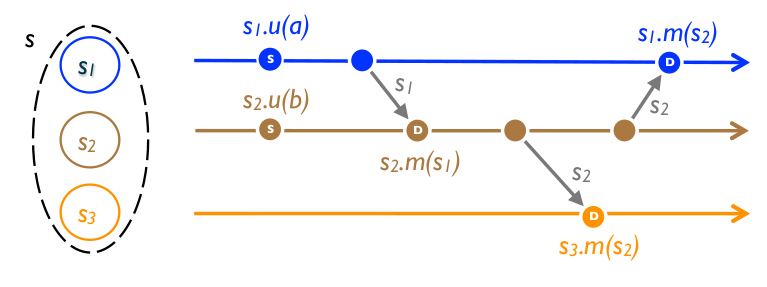
\includegraphics[width=0.8\textwidth]{crdt-state}
  \grayRule
  \caption[Replikation von zustandsbasierten \glspl{CRDT}]{Replikation von zustandsbasierten \glspl{CRDT}, Quelle: ~\cite{crdt_shapiro2}}
  \label{fig:crdt-state}
\end{figure}
%
Die drei Kreise auf der linken Seite repräsentieren drei identische Datensätze auf drei Geräten. Die Datensätze \it{S1} und \it{S2} werden zeitgleich mit unterschiedlichem Kontent aktualisiert.
Kurz darauf, weiter rechts im Bild, sendet \it{S1} seinen neuen Status an \it{S2}.
\it{S2} führt die beiden Status, den von \it{S1} empfangenen und den eigenen, aktualisierten, in der \tt{merge} Funktion $m$ zusammen.
Dann schickt es den eigenen, neuen Status an \it{S3} und \it{S1}, welche ebenfalls den empfangenen mit dem eigenen Status zusammenführen. Beide Aktualisierungen haben nun alle Geräte erreicht und alle Daten sind identisch.\\\\
%
Damit die Replikation konfliktfrei funktioniert müssen einige Voraussetzungen erfüllt sein.
Der Status, den ein \gls{CRDT} hat muss ein Semi--Gitter, also eine geordnete Menge abbilden.
Die Aktualisierungen müssen zunehmend sein, ein Status kann beispielsweise eine Zahl sein und die Aktualisierung ist die Operation die sie inkrementiert.
Die \tt{merge} Funktion muss die kleinste obere Grenze der letzten Aktualisierung berechnen.
Nur wenn ein Objekt diese Eigenschaften erfüllt, ist es dem \gls{CRDT} zugehörig ~\cite{crdt_shapiro2}
%
%
%
\subsub{Operationsbasierter Ansatz}
Wenn ein Replikat eine Aktualisierung von einem Client empfängt, wird es ebenfalls zuerst auf den lokalen Status angewandt.
Im Gegensatz zum zustandsbasiertem Ansatz wird nicht der gesamte Status des Replikats gesendet, sondern nur der Aktualisierungsvorgang.
Ein weiterer Unterschied ist das Fehlen der \tt{merge} Funktion. Statt ihrer gibt es im operationsbasierten Ansatz zwei \tt{update} Methoden: eine vorbereitende Aktualisierungsfunktionen und eine ausführende. Erstere wird auf dem Replikat angewandt, umgehend gefolgt von der zweiten.
Über ein Kommunikationsprotokoll wird die Aktualisierung an alle anderen Replikas asynchron versendet.
Über das Protokoll wird sichergestellt, dass die Nachricht nur einmal überliefert wird.
Die restlichen Replikas wenden die Operation mit der ausführenden Aktualisierungsmethode auf sich an~\cite{crdt_shapiro2}.
Die folgende Abbildung stellt eine operationsbasierte Replikation mit drei Geräten dar.
%
\begin{figure}[H]
  \centering
  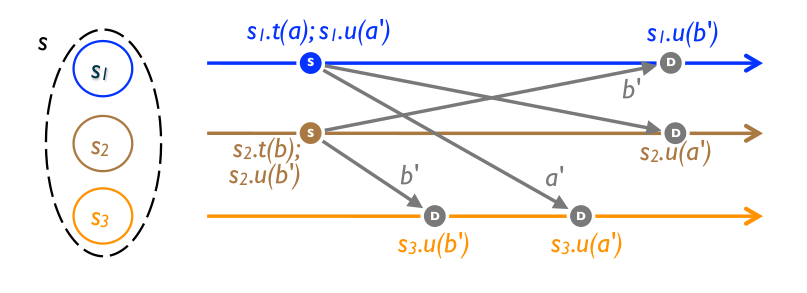
\includegraphics[width=0.8\textwidth]{crdt-op}
  \grayRule
  \caption[Replikation von Operationsbasierten \gls{CRDT}]{Replikation von Operationsbasierten \glspl{CRDT}, Quelle: ~\cite{crdt_shapiro2}}
  \label{fig:crdt-op}
\end{figure}
%
Die drei Kreise auf der linken Seite repräsentieren drei identische Datensätze auf drei Geräten. Die Datensätze \it{S1} und \it{S2} werden zeitgleich mit unterschiedlichem Kontent aktualisiert.
Sowohl \it{S1} also auch \it{S2} wenden die vorbereitende Aktualisierungsmethode $t$ auf sich an.
Dann, mit dessen Ergebnis, die ausführende $u$.
Sofort senden beide Relikas die Aktualisierung an alle anderen, welche ebenfalls die ausführende Aktualisierungsmethode $u$ auf sich anwenden.\\\\
Die Voraussetzung für eine konfliktfreie Replikation sind hier kommuntative Aktualisierungen.
%Wenn $s$ der Status ist und $u$ die Aktualisierungsmethode, muss $s \bullet u \bullet u' \equiv s \bullet u' \bullet u$ gelten.
Nur so spielt die Reihenfolge in der die Aktualisierungen bei den Replikaten ankommen, keine Rolle -- das Ergebnis ist dasselbe ~\cite{crdt_shapiro2}.\\\\
Umgesetzte \glspl{CRDT} sind zum Beispiel Counter, ein Datenobjekt das zum Zählen verwendet wird. Es gibt einen, der nur hochzählen kann und eine andere Variante die auch die Subtraktion unterstützt.
Weitere \glspl{CRDT} sind Sets, eine Listenrepräsentation ohne Duplikate. Auch hier gibt es eine Variante mit der nur Daten hinzugefügt werden können und eine die auch das Entfernen der Daten erlaubt ~\cite{crdt_shapiro}.
%
%CRDTs befassen sich mit einem interessanten und grundlegendem Problem in verteilten Systemen, haben jedoch eine wichtige Einschränkung:
%"Da ein CRDT konstruktionsbedingt keinen Konsens verwendet, hat der Ansatz starke Einschränkungen; Dennoch sind einige interessante und nicht-triviale CRDTs bekannt" ~\cite{crdt_shapiro2}.
%Die Einschränkung ist, dass die CRDT-Adresse nur einen Teil des Problemraums betrifft, da nicht alle möglichen Aktualisierungsoperationen kommutativ sind und daher nicht alle Probleme in CRDTs umgewandelt werden können.
%
%Alas, everything in programming is trade-offs, so what do we trade for being able to have conflict-free data structures? Well, they are specialised data structures, like sets and counters, and not generic object representations like JSON, so we’ll have to buy into a whole world of these specialised data structures, and maybe we have hard time mapping our application objects to them. 
%
% Couch Pouch
%
\hyperref[chap:couch]{CouchDB} ist ein quelloffenes, dokumentenorientiertes \gls{DBMS} mit einem integrierten Replikationsprotokoll.\\
Die Aufgabe der Replikation von CouchDB ist die nahtlose, direkte Datensynchronisation zweier oder mehrerer Datenbanken.
CouchDB verwendet Replikation um Änderungen an Dokumenten zwischen einzelnen Knoten zu synchronisieren.
%. These databases can live on the same server or on two different servers—CouchDB doesn’t make a distinction. If you change one copy of the database, replication will send these changes to the other copy. 
Hierbei werden nur die Dokumente übertragen, die neu sind oder sich geändert haben.
Die Replikation in CouchDB erfolgt schrittweise. Alle Änderungen an Dokumenten werden periodisch zwischen den Servern kopiert.
Wenn der Replikationsprozess unterbrochen wurde weil eine Datenbank keinen Internetzugang hat, haben zwei sich replizierende Datenbanken unterschiedliche Daten gespeichert -- einen inkosistenten Status.
Bei wieder bestehender Internetverbindung wird die Replikation erneut ausgelöst und CouchDB setzt an dem Punkt an dem es ausgefört hat, die Arbeit fort.\\\\
%
Das Besondere an CouchDB ist, dass es darauf ausgerichtet ist, Konflikte vernünftig zu behandeln statt anznehmen es träten keine auf.
Das interne Replikationssystem besitzt eine automatische Konflikterkennung und --lösung.\\
Wichtig für diesen Mechanismus sind die Revisionsnummern.
Dokumente werden mit Revisionsnummern versioniert. Mit jeder Aktualisierung bekommt es eine neue Revision, die neben der alten gespeichert wird (vgl. \cite{couchDB} S. 15ff \& S. 150ff). 
Eine Revisionsnummer in CouchDB kann wie folgt aussehen \tt{2-5560348cec1b08c3d53e1508b4a46868} und ist in zwei Bereiche zu teilen. Die Zahl vor dem \tt{-} erhöht sich mit jeder neuen Revision des Dokuments, also mit jeder Aktualisierung. Alles hinter dem Strich ist ein md5--\gls{Hash} aus dem Dokumenteninhalt, den Dateianhängen und dem \tt{\_deleted} Attribut\footnote{ Dokumente werden in CouchDB nicht ohne Weiteres gelöscht. Stattdessen werden sie als solches markiert.}. Jede Revision hat außerdem eine Liste von vorherigen Revisionen.\\\\
Hat ein Dokument durch gleichzeitiges Bearbeiten in zwei unterschiedlichen Datenbanken dieselbe Revisionsnumer, erkennt CouchDB den Konflikt und markiert indem das Dokument das Attribut \tt{\_conficts} mit dem Wert \tt{true} bekommt. Dann entscheidet CouchDB, welche Version gewinnt und welche verliert.
CouchDB wird nie zwei Versionen zusammenführen. Das muss in der Anwendung implementiert sein.
Die Entscheidung darüber, welche Version gewinnt erfolgt über den Längenvergleich der Revisionslisten. Die Version mit der längsten Liste aus vorherigen Revisionen gewinnt. Sind beide Listen gleich lang, gewinnt die Revision die laut alphabetischer Sortierung am größten ist.\\
Auch wenn CouchDB die gewinnende und die verlierende Revision festlegt, werden beide Versionen gespeichert. Die gewinnende Revision wird als letztes gespeichert, die verlierende davor. Diese Konfliktlösungsstrategie wird auf allen CouchDB Instanzen angewandt, weswegen dazu keine Internetverbindung notwendig ist. Dadurch, dass alle Instanzen denselben Algorithmus verwenden werden die Revisionen immer in identischer Reihenfolge gespeichert. Dadurch bleiben die Daten konsistent.\\
Jetzt kann im Entwicklungsprozess der Anwendung entschieden werden, wie mit den Konflikten umgegangen wird.
Es kann aus beiden Version eine festgelegt werden, die behalten wird oder es können beide zusammengeführt werden (vgl. \cite{couchDB} S. 153ff).
%
\subsub{Eventual Consistency}
\todo{Das muss noch woanders hin. oder raus}\\
Das \gls{CAP} Theorem, veranschaulicht in \autoref{fig:cap}, besagt, dass jedes System mit dem Daten über das Netzwerk gesendet werden, nur zwei von den drei möglichen Eigenschaften, Konsistenz, Verfügbarkeit und Partitionstoleranz, garantieren kann.
Konsitzenz der gespeicherten Daten bedeutet, es muss sichergestellt werden dass nach Abschluss der Transaktion auch alle Replikate des manipulierten Datensatzes aktualisiert werden. Der Datensatz ist in jeder Datenbank identisch.
%
\begin{figure}[H]
  \centering
  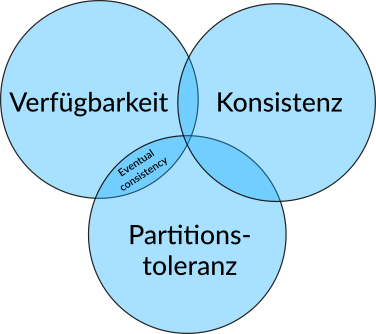
\includegraphics[width=0.6\textwidth]{cap}
  \grayRule
  \caption{Das CAP Theorem}
  \label{fig:cap}
\end{figure}
%
Das System ist besitzt eine hohe Verfügbarkeit wenn alle Anfragen an das System stets beantwortet werden. Die Verfügbarkeit ist gering, wenn die Antwortzeiten des Systems lang sind.
Partitionstoleranz ist gleichzusetzen mit Ausfalltoleranz. Die Datenbank kann auf mehreren Servern verteilt sein. Trotzdem ein Server oder eine Partition ausfällt, kann das System weiterhin funktionieren.\\
Eventual Consistency kommt häufig bei verteilten Datenbanken zur Anwendung und stellt die Konsitenz der Daten nach einem gewissen Zeitfenster sicher (vgl. ~\cite{couchDB} S. 11 ff.). 
% Wenn Verfügbarkeit Priorität hat, können wir Clients die Daten zunächst auf einen Knoten schreiben lassen, ohne darauf zu warten, dass die anderen Knoten synchronisiert werden.
% Wenn die Datenbank weiß, wie sie mit dieser Situation umzugehen hat, sind die Daten irgendwann „letztendlich konsistent“ — allerdings unter Aufgabe der Hochverfügbarkeit der Daten.
% Für viele Anwendungen ist das ein erstaunlich guter Kompromiss.
% Das CouchDB Replikationsmodell erlaubt eine nahtlose, direkte Datensynchronisation zwischen beliebig vielen Geräten.
% Das CouchDB Replikationsprotokoll ist in CouchDB selbst implementiert, das die Serverkomponente abdeckt~\cite{couch}.
%content addressable versions: Idee: Nimm den Objektinhalt (content) und jag ihn durch eine \gls{Hash}funktion\\
%Zuverlässige Synchronisation von Datenbanken auf verschiedenen Geräten.
%Verteilung der Daten über ein Cluster von DB-Instanzen die jeweils einen Teil des requests beantworten (Lastverteilung) und \b{Spiegelung} der Daten über geografisch weit verteilte Standorte.\\
% Durch die inkrementelle (schrittweise) Arbeitsweise kann CouchDB genau dort weitermachen wo es unterbrochen wurde wenn während der Replikation ein Fehler auftritt, beispielsweise durch eine ausfallende Netzwerkverbindung
% \it{Es werden auch nur die Daten übertragen, die notwendig sind, um die Datenbanken zu synchronisieren.}\\
%
%Diese Art von Konflikten sollten von Menschen gelöst werden. Nur so kann sichergestellt werden, dass die korrekte Änderung gespeichert wird und keine Daten verloren gehen.
%
%Dann gibt es das PouchDB-Projekt, das dasselbe Protokoll in JavaScript implementiert, das auf Browser- und Node.js-Anwendungen abzielt. das deckt Ihre Kunden und dev-Server ab.
%Schließlich gibt es Couchbase Mobile und Cloudant Sync, die auf iOS und Android laufen und das CouchDB Synchronisationsprotokoll in Objective-C bzw. Java implementieren.}\\

%
% Frameworks / Bibliotheken
%
\chapter{\label{chap:state}Bestehende offlinefähige Technologien}
Um eine Webapplikation offlinefähig zu machen, müssen alle Daten auf dem Client gespeichert werden und von diesem zu jeder Zeit abrufbar sein.
Für Anwendungen mit einer serverseitigen Datenbank ist die Synchronisation der Daten zwischen Server und Client notwendig.\\
Es gibt verschiedene Technologien, die sich diesen Problematiken widmen.
Diese umfassen Bibliotheken und Frameworks, die die Entwicklung offlinefähiger Anwendungen unterstützen, sowie Datenbanklösungen. In den nächsten Punkten werden einige dieser Technologien näher beschreiben.
%
% webpack offline-plugin
%
\section{Offline plugin für webpack}
Webpack ist ein JavaScript `Bundler` und bündelt alle Skripte, Bilder und \gls{Assets} für die Verwendung in Browsern.\\
Das Offline Plugin bietet Offlinefunktionalität für Webpackprojekte indem es die gebündelten, also von Webpack generierten \gls{Assets} cached.
Dazu benutzt es intern den ServiceWorker und AppCache als Reserve, für den Fall dass der Browser ServiceWorker nicht unterstützt~\cite{webpack-gh}.\\
Auch ungebundelte \gls{Assets} können über das Plugin gecached werden. Diese Dateien müssen dann in den Optionen explizit angegeben werden. Auch der ServiceWorker und der AppCache lassen sich über die Optionen konfigurieren oder auch ausschalten~\cite{webpack-opt}.\\
Es werden allerdings nur die \gls{Assets} und nicht die von BenutzerInnen generierten Daten gecached. Diese müssen manuell im gespeichert werden.
%
% redux-offline
%
\section{\label{sub:reduxoffline}Redux Offline}
%``Persistenter Redux store für \it{reasonaboutable}\tm ~Offline-First Anwendungen``. \\
Redux Offline kann nur zusammen mit Redux verwendet werden~\cite{redux-req}. Deswegen ist für die Verwendung von Redux Offline die Implementierung von Redux vorausgesetzt.
%
% Redux
%
% Alles beginnt mit dem Aufruf von \tt{store.dispatch(action)} von jeder beliebigen Stelle in der Anwendung. Die Aktion die beschreibt was passiert heißt \tt{toggleEdit} und sieht im Beispiel des Ansichtswechsels aus wie in Zeile drei bis fünf.\\
% Der \tt{Store} ruft nun den \tt{Reducer} auf
\sub{Redux}
Redux ist eine JavaScript Bibliothek die Probleme im Zusammenhang mit dem \it{Zustand} einer Anwendung löst.
Redux ist eine Bibliothek zur Zustandsverwaltung in JavaScriptanwendungen.
Es gibt einen zentralen Ort, in dem der \it{Zustand} der App gespeichert ist, auf den von jeder Komponente aus zugegriffen werden kann.
Dieser Ort wird \sc{Store} genannt und jede Applikation hat genau einen davon. 
Als einzige Informationsquelle für den Store als zentralen Speicher dienen Aktionen. 
Sie senden Daten von der Anwendung mittels \tt{store.dispatch()} an den \sc{store} und beschreiben dabei nicht wie etwas passiert, sondern was passiert.
Der dritte wichtige Bestandteil von Redux sind die \sc{Reducer}. Sie spezifizieren wie der Status sich als Reaktion auf die Aktionen ändert~\cite{redux}.\\
Der Datenfluss in der Reduxarchitektur ist unidirektional. Zur Veranschaulichung wird anhand der folgenden Abbildung der Redux Datenfluss beschrieben.
%
\begin{figure}[H]
  \centering
  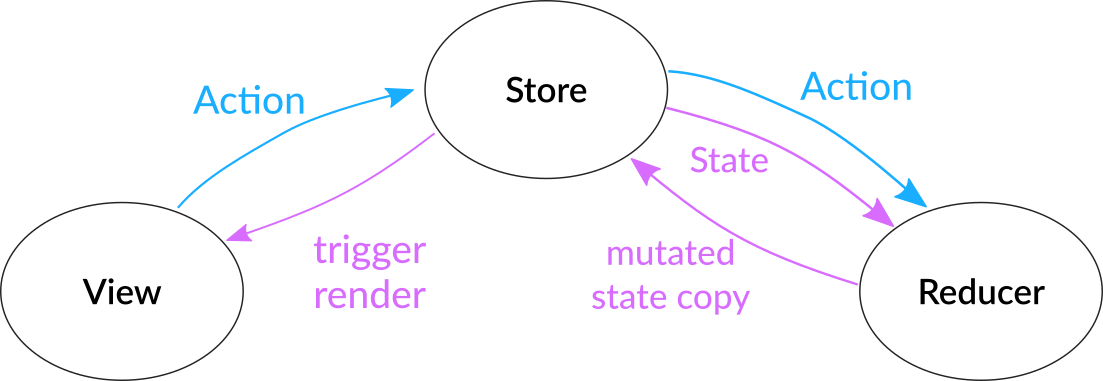
\includegraphics[width=0.8\textwidth]{redux-flow}
  \grayRule
  \caption{Redux Datenfluss}
  \label{fig:rdx-dataflow}
\end{figure}
% 
Zuerst sendet die View eine Aktion an den Store. Dieser empfängt die Aktion und schickt sie zusammen mit dem Applikationsstatus an den \sc{Reducer}.
Der \sc{Reducer} erstellt eine Kopie des Status, verändert diese und schickt sie wieder zurück an den \sc{Store}. Der \sc{Store} ersetzt nun den alten mit dem neuen Status und löst ein erneutes Rendern der View aus.
% 
% Redux Offline
% 
\sub{Redux Offline}
Redux Offline erweitert Redux um einen persistenten \sc{Store} mit Offline-First Technologie und  ist kompatibel mit allen *View Frameworks wie React\footnote{JavaScript Bibliothek: \url{https://reactjs.org/}}, Vue\footnote{JavaScript Framework: \url{https://vuejs.org/}}, oder Angular\footnote{JavaScript Framework: \url{https://www.angular.io}}~\cite{redux-offline-compabilaty}.
Es umfasst unter Anderem netzwerkfähige \gls{API}-Aufrufe, das Persistieren des Zustands der Anwendung, das speichern von Aktionen, die Behandlung von Fehlern und erneute Versuche die Verbindung wieder herzustellen.
Redux Offline verspricht nicht, die Webanwendung komplett offlinefähig zu machen. Um \gls{Assets} zwischenzuspeichern, muss zusätzlich noch ein ServiceWorker implementiert sein ~\cite{redux-offline-gh}.\\
Die Idee hinter Redux Offline ist, dass der Redux \sc{Store} die Datenbank ersetzt~\cite{redux-offline}. Bei jeder Änderung wird der Redux \sc{Store} auf dem Datenträger gespeichert, und bei jedem Start automatisch neugeladen. Für das Speichern der Daten in einer lokalen Datenbank wird intern \hyperref[sub:reduxpersist]{Redux Persist} verwendet.\\\\
Eine mit Redux Offline erstellte Anwendung funktioniert ohne weitere Codeimplementierung offline im Lesemodus, da das Lesen und Schreiben aus der lokalen Datenbank bereits eigebunden ist.
Damit die Anwendung auch im Schreibmodus offline funktioniert, müssen einige Anpassungen vorgenommen werden.
Sämtliche Daten der Anwendung können nur über Aktionen manipuliert werden. 
Alle netzwerkgebundenen Aktionen werden  in einem \sc{store}internem \gls{Queue} gespeichert und müssen mit einem Metaattribut dekoriert werden um offline arbeiten zu können. Durch die Metaattribute weiß die Anwendung was vor der eigentlichen Ausführung der Aktion und was danach zu tun ist. 
Es gibt drei Metadaten die Redux Offline interpretieren kann:\\
\tt{meta.offline.effect} - Die initiale Aktion wird ausgeführt. Hier kann eine URL angegeben werden die Redux Offline anfragen soll.\\
\tt{meta.offline.commit} - Hier wird die Aktion definiert die ausgeführt wird sobald die Netzwerkanfrage erfolgreich ist.\\
\tt{meta.offline.rollback} - Hier kann die Aktion angegeben werden, die bei  permanent fehlgeschlagener Internetverbindung oder wenn der Server einen Serverfehler zurückgibt gefeuert wird.
Dann fügt Redux Offline dem \sc{Appstate} automatisch ein \tt{offline} Objekt hinzu. Dort wird unter anderem ein Array namens \tt{outbox} verwaltet wird.
Dieses Array repräsentiert den \gls{Queue}. Hier werden die Aktionen inklusive Metadaten gespeichert, um bei bestehender Internetverbindung abgearbeitet zu werden~\cite{redux-offline-docs}.
Die von Jani Eväkallio erstellte Grafik \ref{fig:redux-offline} veranschaulicht die oben erklärte Architektur.\\
%
\begin{figure}[h]
  \centering
  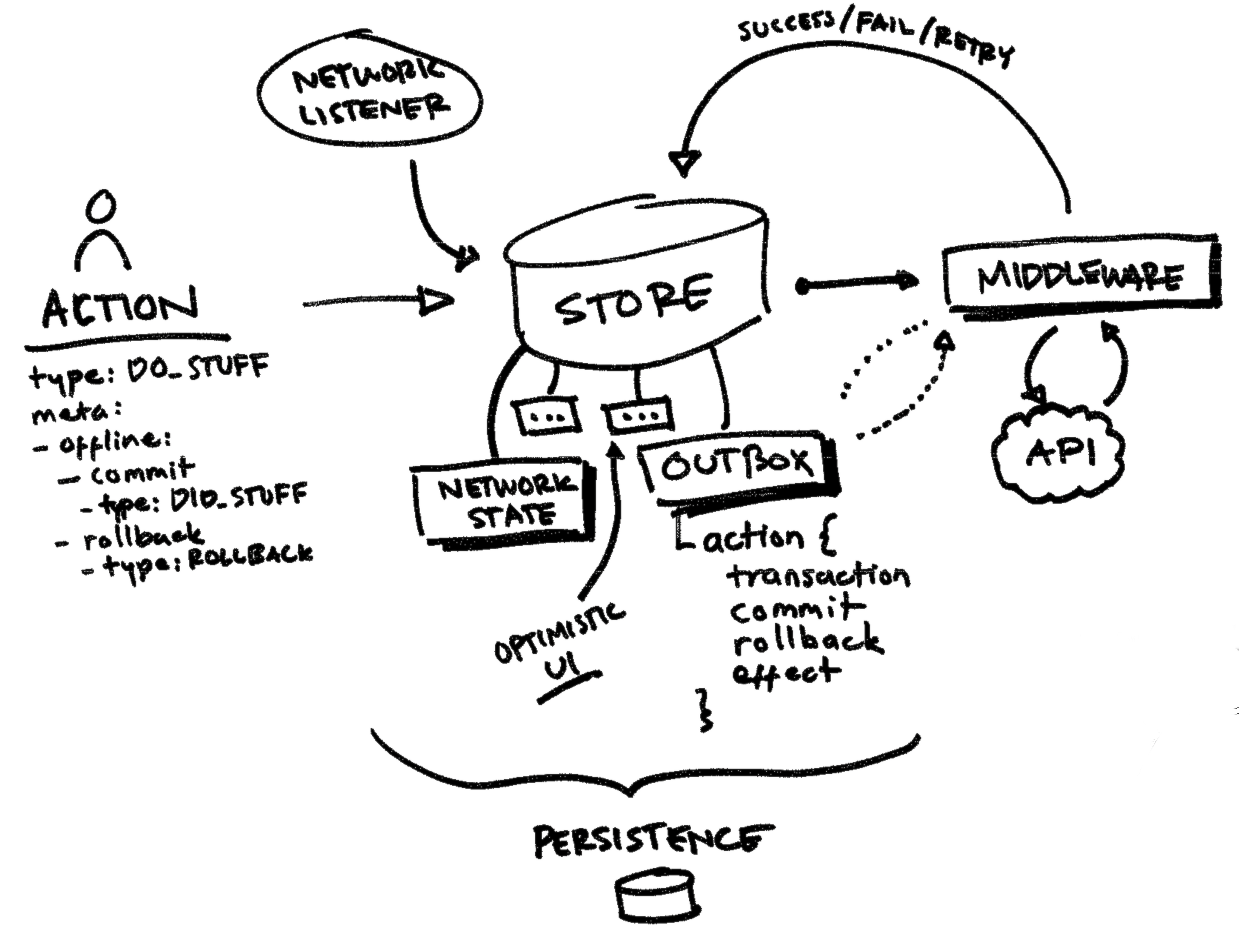
\includegraphics[width=0.8\textwidth]{redux-offline-new}
  \grayRule
  \caption[Redux Offline]{Redux Offline Architektur~Quelle:~\cite{redux-offline}}
  \label{fig:redux-offline}
\end{figure}
%
Links ist eine Aktion zu sehen die Zeug machen möchte. Sie hat ein Mateattribut das weitere Aktionen definiert. Eine Aktion für den Erfolg und eine für den Fehlschlag von `DO\_STUFF`.
In der Mitte ist der \sc{Store} zu sehen. Der \sc{Store} kennt den Netzwerkstatus und hat den \gls{Queue} namens \tt{outbox} in dem Aktionen mitsamt ihrer Metafelder gespeichert werden. Rechts befindet sich das \gls{API}, das über die \gls{Middleware} mit dem \sc{Store} redet.\\
Wird die Aktion 'DO\_STUFF' gefeuert gelangt sie in den \sc{Store}, damit dieser den \sc{AppState} aktualisieren kann, und wird ersteinmal im \gls{Queue} gespeichert. Ist die Anwendung online, wird sie sofort abgearbeitet. Wenn nicht wird sie dort gespeichert bis die Anwendung wieder eine Verbindung zum Internet hat.   
% \subsub{Konflikte}
%
% redux persist
%
\sub{\label{sub:reduxpersist}Redux Persist}
Redux Persist ist eine Bibliothek, die als Wrapper für den Redux Store funktioniert. Mit Redux Persist wird der \tt{state} automatisch lokal, per default im LocalStorage, gespeichert~\cite{redux-persist}.
Es kann konfiguriert werden wo die Daten gespeichert werden. Hier gibt es diverse Möglichkeiten wie zum Beispiel im SessionStorage, per localForage oder in Dateisystemen~{redux-persist-gh}. LocalForage ist eine Bibliothek mit der Daten in IndexedDB, WebSQL gespeichert werden können. Wenn der Browser die Speichermöglichkeiten nicht unterstützt, wird der LocalStorage genommen~\cite{localforage}.\\
Es ist auch möglich einen eigenen Speicher zu konfigurieren. Die einzige Voraussetzung hierfür ist, das \gls{API} muss die Standardmethoden \tt{setItem}, \tt{getitem} und \tt{removeItem} implementieren und Promises unterstützen~\cite{redux-persist-gh}.
%
% redux optimist
%
% \sub{redux-optimist}
%
% react-native-offline
%
\sub{react-native-offline}
React Native = JavaScript React Framework um native, mobile Apps zu bauen. blabla\\
Behandelt online/offline Verbindung. Kann die Internetverbindung auch regelmäßig prüfen\\
Speichert nur den Status online/offline im store. -> erlaubt so unterschiedliches Rendern von Componenten.\\

\tt{const YourComponent = ({ isConnected }) => (\\
  <Text>{isConnected ? 'I am connected to the internet!' : 'Offline :('}</Text>\\
  );\\}\\
  Zusammen mir Redux hat es einen `Mehrwert`:
  Hat dann einen `Offline-\gls{Queue} um Aktionen zu wiederholen (im Intervall) \tt{meta.retry? \textcolor{gray}  {Array of actions which, once dispatched, will trigger a dismissal from the queue}} ~ oder nicht \tt{meta.dismiss? []}.\cite{rn-offline-gh}
  % \cite{rn-offline-medium}

%
% hoodie
%
\section{hoodie}
HOODIE ist eine JavaScript Bibliothek für offlinefähige Webapplikationen, die ein komplettes Backend zur Verfügung stellt. Wird HOODIE für die Entwicklung einer Webanwendung verwendet, muss also lediglich das Frontend implementiert werden. Den Rest erledigt die Bibliothek. Über eine integrierte Programmierschnittstelle kommuniziert die Anwendung mit dem von HOODIE zur Verfügung gestelltem Backend. Über das \gls{API} können unter Anderen BenutzerInnen authentifiziert, Daten gespeichert und synchronisiert werden~\cite{hoodie}.\\
Anhand der Abbildung \ref{fig:hoodie} wird erklärt wie HOODIE funktioniert.
\begin{figure}[H]
  \centering
  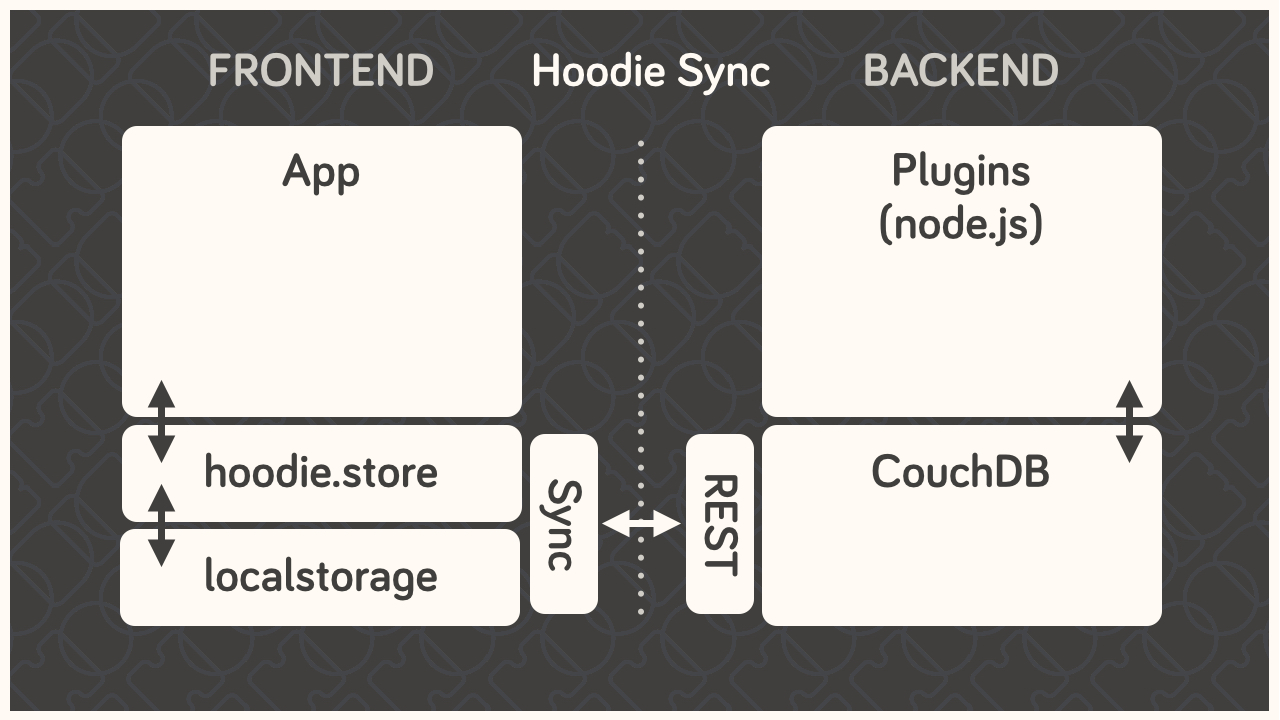
\includegraphics[width=0.8\textwidth]{hoodie}
  \grayRule
  \caption[HOODIE Architektur]{HOODIE Architektur~Quelle:~\cite{hoodie-how}}
  \label{fig:hoodie}
\end{figure}
Im Frontend--Bereicht ist die App zu sehen die über das HOODIE \gls{API} mit dem lokalen Speicher kommuniziert. Die Anwendung spricht niemals direkt mit dem Server oder der Datenbank. Für die lokale Speicherung der Daten benutzt HOODIE intern PouchDB, was wiederum IndexedDB verwendet. Durch das lokale Speichern sind die Daten auch offline verfügbar. Dann werden über eine \gls{REST} Schnittstelle mit einer CouchDB synchronisiert. CouchDB ist eine Datenbank mit der Superkraft des Synchronisierens und in HOODIE haben alle AnwenderInnen ihre eigene private CouchDB. Hinter der Datenbank befindet sich ein kleiner Server der auf die Daten in der CouchDB reagiert, die wiederum die Änderungen an den Client schickt ~\cite{hoodie-how}.
So können NutzerInnen nur auf ihre eigenen Daten zugreifen. Wenn es mehrere Geräte gibt, die mit einem Account assoziiert werden, werden die Änderungen von einem Gerät zuerst auf die serverseitige CouchDB synchronisiert, um dann von dort in die lokalen Datenbanken der anderen Geräte zu gelangen.\\
Dadurch, dass das Frontend und das Backend nicht direkt miteinander sprechen, ist die Funktionalität beider Komponenten auch dann gewährleistet, wenn die Verbindung unterbrochen wird.
%
% realm
%
\section{\label{sub:realm}Realm}
Realm ist eine Backendtechnologie für mobile Anwendungen und umfasst die Realm--Datenbank und den Realm Object--Server.
Die Datenbank ist quelloffen, der Object--Server jedoch nicht -- dieser ist außerdem nicht kostenfrei~\cite{realm}.\\
Die Realm--Datenbank ist eine objektorientierte, plattformübergreifende lokale Datenbank die eine Echtzeitsynchronisation mit dem Realm Object--Server bereitstellt.
Der Object--Server fungiert als \gls{Middleware}-Komponente in der mobilen \gls{App} und handhabt unter anderem die Ereignisbehandlung und Datensynchronisation.
Im Zusammenspiel ermöglichen die beiden Technologien die Erstellung von offlinefähigen, kollaborativen, mobilen Anwendungen~\cite{realm_whitepaper}.\\\\
%
%
Zur Offline First--Funktionalität stellt Realm eine umfassende Lösung bereit.
Die lokale Realm--Datenbank unterstützt die Echtzeitsynchronisation von Daten, sodass alle Änderungen sofort automatisch gesendet werden.
Das Synchronisationsprotokoll komprimiert statt dem gesamten Objekt nur die marginalen Änderungen und synchronisiert sie auf dem Endgerät und dem Server.
Zusätzlich zu den Daten werden die spezifischen Operationen erfasst. 
Wird beispielsweise ein Kontakt bearbeitet, wird neben den geänderten Daten die Information \it{update} mitgesendet.
Dank dieser zusätzlichen Information kann der Aktionswunsch genau erfasst werden, sodass das System auftretende Konflikte automatisch auflösen kann.
Das hat zur Folge, dass die Synchronisation keinen manuellen Eingriff bedarf ~\cite{realm_offline_whitepaper}.\\
%
Zusätzlich zu dem \gls{OT}--Algorithmus benutzt Realm vorgegebene Regeln zur automatischen Konfliktlösung.
In Realm gibt es drei Grundregeln, die die hauptsächlichen Aktivitäten abdecken.
Neue Einträge in Listen werden zeitlich sortiert. Für den Fall dass zwei Objekte gleichzeitig zur selben Liste hinzugefügt werden, wird das mit dem neueren Zeitstempel hinter dem älteren Objekt gespeichert.
Löschungen haben immer Vorrang; auch dann, wenn das auf dem einen Gerät gelöschte Objekt auf einem anderen zu einem späteren Zeitpunkt bearbeitet wurde.
Für die Aktualisierungen wird die Konfliktmanagementstrategie \gls{LWW} angewandt, die letzte Aktualisierung gewinnt.
Wird ein Objekt auf zwei Geräten bearbeitet, wird das mit dem neueren Zeitstempel behalten.\\ 
Es besteht auch die Möglichkeit, eigene Regeln zu definieren oder die bestehenden zu überschreiben ~\cite{realm_conflict}.
% Eine Regel könnte zum Beispiel sein, dass alle Änderungen die von der Nutzerin, nennen wir sie Amilia Pond, gemacht werden den Vorrang haben. Das ist keine gute Regel, denn dabei würden definitiv Daten verloren gehen wenn eine andere Person eine andere Änderung an derselben Stelle wie Amilia Pond macht, aber sie soll ja nur als Beispiel dienen.\\
Darüber hinaus läuft die interne Konfliktlösung auf Transaktionsebene ab.
Das heißt, der Vorgang ist nur erfolgreich, wenn er auch vollständig und fehlerfrei ist. Andernfalls wird er zurückgesetzt.
Das gewährleistet die Konsistenz der Daten und verhindert deren Verlust, wenn Änderungen aufgrund einer unterbrochenen Netzwerkverbindung nicht stattfinden können~\cite{realm_offline_whitepaper}.
%
% \section{DerbyJS -- wenn noch Zeit bleibt}
\clearpage
\section{Übersicht}
Alle oben genannten Systeme unterstützen, nach eigener Aussage, die Erstellung offlinefähiger Anwendungen.
Die folgende Tabelle fasst die oben genannten Systeme zusammen und zeigt, inwiefern die Technologien, die in \autoref{chap:offlinefirst} genannten Voraussetzungen an eine Offline First--\gls{App} erfüllen.
\begin{longtable}[c]{@{}
	>{\columncolor[HTML]{CFFCC2}}l llll@{}}
	\toprule
	\multicolumn{1}{p{0.33\textwidth}}{\cellcolor[HTML]{cffcc2}\textbf{Produkt}} &
	\multicolumn{1}{p{0.16\textwidth}}{\cellcolor[HTML]{cffcc2}\textbf{Cachen der\newline \gls{Assets}}} &
  \multicolumn{1}{p{0.2\textwidth}}{\cellcolor[HTML]{cffcc2}\textbf{Lokale\newline Datenspeicherung}} &
	\multicolumn{1}{p{0.2\textwidth}}{\cellcolor[HTML]{cffcc2}\textbf{Datenbank-synchronisation}}\\
  %
  \hline \noalign{\vskip 0.1cm}
	\endfirsthead
	\endhead
	%
\multicolumn{1}{p{0.33\textwidth}}
{\textbf{Offline Plugin für webpack}}
&       
\multicolumn{1}{p{0.16\textwidth}}
{Ja}
& 
\multicolumn{1}{p{0.2\textwidth}}
{ -- }
&                                                                                         
\multicolumn{1}{p{0.2\textwidth}}
{ -- }\\
\midrule
% ----------------------------------------------
\multicolumn{1}{p{0.33\textwidth}}
{\textbf{Redux Offline}}
&       
\multicolumn{1}{p{0.16\textwidth}}
{ -- }
& 
\multicolumn{1}{p{0.2\textwidth}}
{Ja}
&                                                                                         
\multicolumn{1}{p{0.2\textwidth}}
{ -- }\\
\midrule
% ----------------------------------------------
\multicolumn{1}{p{0.33\textwidth}}
{\textbf{React Native Offline}}
&       
\multicolumn{1}{p{0.16\textwidth}}
{ -- }
& 
\multicolumn{1}{p{0.2\textwidth}}
{Ja}
&                                                                                         
\multicolumn{1}{p{0.2\textwidth}}
{ -- }\\
\midrule
% ----------------------------------------------
\multicolumn{1}{p{0.33\textwidth}}
{\textbf{HOODIE}}
&       
\multicolumn{1}{p{0.16\textwidth}}
{ -- }
& 
\multicolumn{1}{p{0.2\textwidth}}
{Ja}
&                                                                                         
\multicolumn{1}{p{0.2\textwidth}}
{Ja}\\
\midrule
% ----------------------------------------------
\multicolumn{1}{p{0.33\textwidth}}
{\textbf{Realm}}
&       
\multicolumn{1}{p{0.16\textwidth}}
{ -- }
& 
\multicolumn{1}{p{0.2\textwidth}}
{Ja}
&                                                                                         
\multicolumn{1}{p{0.2\textwidth}}
{Ja}\\
% ----------------------------------------------
	% end
	\bottomrule \cellcolor[HTML]{FFFFFF}
	\vspace{0.1cm}\\
	\noalign{\hspace{0.0525\textwidth}\grayRule}
	\caption{Übersicht der offlinefähigen Technologien}
	\label{tab:stoa}\\
\end{longtable}
%
%
%
Das Offline--Plugin für webpack cacht lediglich die \gls{Assets} einer Anwendung, was sämtliche andere Technologien in dieser Tabelle jedoch nicht tun.
Hierbei sollte beachtet werden, dass React Native Offline und Realm für die Entwicklung von mobilen Anwendungen gemacht sind.
In mobilen \glspl{App} ist das Cachen der \gls{Assets} nicht notwendig, denn alle Dateien die zur Ausführung notwendig sind, werden bei der Installation auf dem Gerät gespeichert.\\
Die lokale Speicherung der von den NutzerInnen generierten Daten wird von allen Technologien, bis auf das Plugin für webpack, unterstützt.
Hierbei unterscheiden sich die Speicherorte der Daten.
Eine Synchronisation zu einer Serverdatenbank stellen allein HOODIE und Realm bereit.
Die restlichen Technologien stellen die Verwendung einer Serverdatenbank frei.
\chapter{\label{chap:szenarien}Szenarien}
Alle in Kapitel \ref{chap:state} angeführten Technologien haben die Unterstützung der Erstellung von offlinefähigen Anwendungen gemeinsam.
Prinzipiell sollte eine Offline First Anwendung in der Lage sein, mit fehlender Internetverbindung zu funktionieren und mit auftretenden Konflikten so umgehen zu können, dass keine Daten verloren gehen.
Sie muss die Fälle behandeln können, die sich aus den folgenden Szenarien ergeben.
Dafür werden zunächst Szenarien in der Netzwerkübetragung als Voraussetzung für die der Konfliktentstehung aufgezeigt.
%
% Netzwerk Szanarien   --------------------------------------------------------
%
\section{\label{sec:netszenarien}Szenarien bei der Datenübertragung}
Im einfachen Anwendungsbeispiel einer Kontaktliste gibt es zwei Parteien die miteinander interagieren: die Anwendung als Client und der Server. Immer wenn beide Parteien miteinander kommunizieren möchten, kann eine der beiden offline sein.
Der Client könnte zum Beispiel, ohne dass eine Technologie implementiert ist die Offlinestatus behandelt, einen Kontakt erstellen wollen. Der Kontakt kann aber nicht erstellt werden, da kein Netzwerk verfügbar ist.\\
`Client push` steht dafür, dass der Client etwas an den Server schickt. `Server push/Client pull` beschreibt den Fall in dem der Client Daten vom Server anfragt, oder der Server Push-Nachrichten an den Client sendet.\\
\todo{Peer-to-Peer? Als Abstraktion über dem Client-Server-Modell. Ein Client = mal Server, mal Client-Rolle}
%
% \todo{Erstellen = erstellen, aktualisieren, löschen}
\begin{description}[leftmargin=0.5cm,style=nextline]
% client push
\item[Szenario C0 -- Client push:]
Der Client erstellt einen Adressbucheintrag, hat den Status \sc{online} und der Server ist erreichbar. Sowohl Anfrage als auch Antwort sind erfolgreich. Der Kontakt wird erfolgreich erstellt.\\
\item[Szenario C1 -- Client push:]
Der Client erstellt einen Adressbucheintrag, hat den Status \sc{offline} und der Server ist nicht erreichbar. Die Anfrage schlägt fehl.\\
\item[Szenario C2 -- Client push:]
Der Client erstellt einen Adressbucheintrag und hat den Status \sc{online}. Die Anfrage wird gestartet und währenddessen bricht die Internetverbindung ab. Die Anfrage `wartet` bis ein Timeout getriggert wird und schlägt dann fehl. Wärend des Wartens ist der Client blockiert.\\
% \item[Szenario C3 -- Client push:]
% Der Client erstellt einen Adressbucheintrag und hat den Status \sc{online}. Die Anfrage wird gestartet und währenddessen bricht die Internetverbindung ab. Die Anfrage ist teilweise erfolgreich. Nur ein Teil der Telefonnummer kommen beim Server an.\\
% client pull / server push
\item[Szenario S0 -- Server push/Client pull:]
Der Client fordert eine Liste aller gespeicherten Kontakte vom Server an, hat den Status \sc{online} und der Server ist erreichbar. Sowohl Anfrage als auch Antwort sind erfolgreich. Die Liste wird komplett ausgeliefert.\\
\item[Szenario S1 -- Server push/Client pull:]
Der Client fordert eine Liste aller gespeicherten Kontakte vom Server an. Dieser hat den Status \sc{offline} und ist nicht erreichbar. Die Antwort schlägt fehl.\\
\item[Szenario S2 -- Server push/Client pull:]
Der Client fordert eine Liste aller gespeicherten Kontakte vom Server an und hat den Status \sc{online}.
Während der Server antwortet, bricht die Internetverbindung ab. Die Antwort `wartet` bis ein Timeout getriggert wird und schlägt dann fehl.
Wärend des Wartens ist der Client blockiert.\\
\item[Szenario S3 -- Server push/Client pull:]
Der Client fordert eine Liste aller gespeicherten Kontakte vom Server an und hat den Status \sc{online}.
Während der Server antwortet, bricht die Internetverbindung ab. Die Antwort ist teilweise erfolgreich.
Nur ein Teil der angefragten Daten kommt beim Client an.
\end{description}
%
%
In den obigen Szenarien wird nicht beschrieben warum die Verbindung zwischen den beiden Parteien abbricht. Dies kann verschiedene Gründe haben.
Um nur einige Beispiele zu nennen: Eine langsame Internetverbindung, oder eine Fahrt durch einen Tunnel kann ein Timeout während einer Aktion hervorrufen.
Ein auf einer Baustelle gekapptes Kabel oder ein Stromausfall kann zu zeitweise vollständigem Internetverlust führen.
Genausogut kann es jedoch sein, dass der Server kaputt oder nicht erreichbar ist. Es gibt meherere Gründe dafür, dass die beiden Parteien nicht mehr miteinander kommunizieren können.

Die Abbildung \ref{fig:szenarien} veranschaulicht die beschriebenen Situationen, die bei der Übertragung von Daten über das Netzwerk eintreten können.
Die Felder in lila beschreiben die Szenarien bei denen der Client etwas an den Server schickt.
Die blauen Felder auf der rechten Seite zeigen solche Szenarien, die eintreten können wenn der Server etwas an den Client sendet.
Die Sechsecke stehen für die Ausgangssituationen, die Kreise repräsentieren die Szenarien und die Rechtecke die daraus resultierenden Fälle.
\begin{figure}[H]
  \centering
  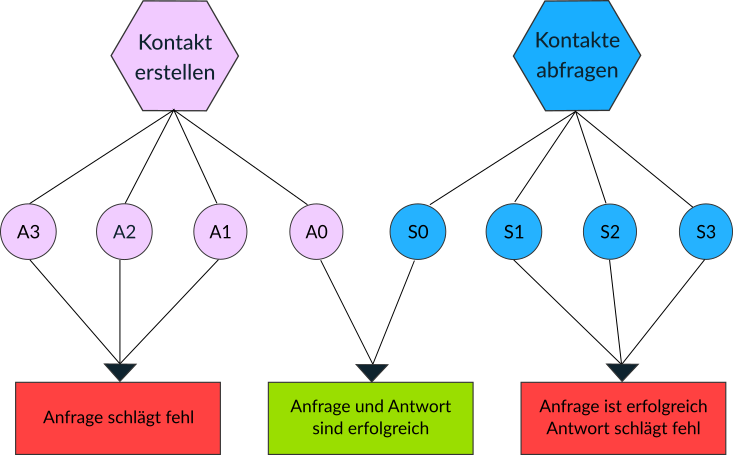
\includegraphics[width=0.8\textwidth]{Szenarien}
  \grayRule
  \caption{Szenarien bei der Datenübertragung über das Netzwerk}
  \label{fig:szenarien}
\end{figure}

%
% ERGEBNIS
%
\subsubsection*{Ergebnis}
Da die Szenarien \it{C0} und \it{S0}, \it{C1} und \it{C2} sowie \it{S1}, \it{S2} und \it{S3} zusammengefasst werden können, ergeben sich aus den sieben Szenarien die drei nun aufgezählten Fälle.
\begin{itemize}
  \item Fall a: Anfrage und Antwort sind erfolgreich.
  \item Fall b: Anfrage ist nicht erfolgreich
  \item Fall c: Anfrage ist erfolgreich, Antwort schlägt fehl
\end{itemize}
Von den erarbeiteten Fällen sind Fall \it{b} und \it{c} für die Szenarien zur Konfliktentstehung relevant. Die Anfrage schlägt fehl und die Anfrage ist erfolgreich aber die Antwort schlägt fehl.
%
%
% Konflikte   -------------------------------------------------------------
%
\section{\label{sec:konfliktszenarien}Szenarien zur Konfliktentstehung}
Im Anwendungsbeispiel einer kollaborativen Kontaktliste können mehrere Personen die Liste verwalten. Oder eine Person benutzt die Anwendung auf mehreren Geräten, was zum selben Ergebnis führt:
Die Komplexität wird durch mehr Parteien -- beliebig viele Clients -- erhöht.
Jede Person kann alle Einträge jederzeit laden und einzelne erstellen, bearbeiten oder löschen. Bei den Ausführungen der grundlegenden \gls{CRUD} Operarionen kann es bei der Synchronisation der beteiligten Parteien zu Konflikten kommen wenn einer der oben genannten Fälle \it{b} oder \it{c} eintritt und ein Objekt von mehreren Parteien bearbeitet wird.\\\\
Aus einem Interview mit \todo{Jan Lenhardt\footnote{Eine berühmte Person}} ergeben sich unterschiedliche, angewandte Vorgehensweisen Objekte für die Verwendung in verteilten Systemen zu identifizieren und versionieren. Nachfolgend werden diese Vorgehensweisen berücksichtigend, Konfliktszenarien erarbeitet. Es ist zu erwähnen, dass es bei diesen Methoden nicht immer zu Konflikten kommen muss. Da es Thema dieser Arbeit ist, wird für jede Variante nur der ungünstigste Fall, der Konfliktfall aufgeschrieben.
% \note{Damit die Einträge sortiert und gefiltert aus der Datenbank geladen werden können, werden sie mit einem Index versehen. Jeder neue Eintrag bekommt automatisch einen höheren Index. Die aktualisierten Objekte sollen ebenfalls geladen werden, aber keinen neuen Index bekommen. Deswegen gibt es neben dem Datensatz \sc{Adressbucheinträge} zusätzlich den der \sc{Aktualisierungen} mit einem sich automatisch erhöhendem Index \it{und der Referenz zum Adressbucheintrag}. \todo{eigenes Szenario?}. Mit jeder Aktualisierung oder Löschung eines Kontakts wird im Aktualisierungsdatensatz der Index durch einen neuen ersetzt. So hat jede Kontakt-ID eine Aktualisierungs-ID und ein Eintrag wird auch nach mehrmaligem Aktualisieren nicht mehrfach geladen.}\\
%
%
% Footnotes
%
\def \naturalkey {Ein Schlüssel, der sich aus einem Attribut des Objekts ergibt oder sich aus mehreren Attributen zusammensetzt. So könnte ein sprechender Schlüssel von Jean-Luc Picard mit der E-Mail-Adresse picard@enterpise.com beispielsweise `picard@enterprise.com` (E-Mail) oder `Jean-LucPicard` (Zusammensetzung aus Vor- und Nachnamen) sein.}
\def \logicalclock {Eine Logische Uhr ist eine Komponente die dazu dient, dem Datenobjekt einen eindeutigen Zeitstempel zuzuweisen. Die bekanntesten Verfahren für Logische Uhren in verteilten Systemen sind die Lamport-Uhr und die Vektoruhr. Beide verwenden Zähler die sich bei jedem Ereignis erhöhen. Einfach gesagt besteht die Lamport-Uhr aus einem Zeitstempel und einem Zähler, die Vektoruhr aus einem Zeitstempel und einem Vektor -- einer Liste aus Zählern.}
%
%
\begin{description}[leftmargin=0.5cm,style=nextline]
  % ID
  \item[Szenario ID0 -- UUID:]
    Zur Identifizierung eines Adressbucheintrags wird eine \gls{UUID} verwendet. Es wird sowohl auf dem Client als auch auf dem Server ein Kontakt mit dem Namen `Amilia Pond` erstellt.
    Währenddessen tritt Fall \it{b} oder \it{c} ein und beide Parteien können nicht miteinander kommunizieren. Nach der Synchronisation existieren zwei Kontakteinträge mit gleichem Namen, aber unterschiedlicher ID.
    Sie sind voneinander zu unterscheiden und können einzeln behandelt werden.\\
  \item[Szenario ID1 -- sprechender Schlüssel:]
    Zur Identifizierung eines Adressbucheintrags wird ein sprechender Schlüssel\footnote{\naturalkey} verwendet.
    Es wird sowohl auf dem Client als auch auf dem Server ein Kontakt mit dem Namen `Amilia Pond` und dem sprechenden Schlüssel `amiliapond` erstellt. Währenddessen tritt Fall \it{b} oder \it{c} ein.
    Es ist nicht zu ermitteln, ob derselbe Kontakt doppelt angelegt wurde, wenn beide Kontakteinträge sich unterscheiden, welcher der beiden korrekt ist oder ob es sich bei den Einträgen um zwei Personen mit demselben Namen handelt.\\
  %
  %
  % Version
  \item[Szenario V0 -- Versionsnummer:]
    Zur Versionierung eines Adressbucheintrags werden Versionsnummern verwendet. Der Kontakt `Amilia` hat die Version `1.0.0`.
    Sowohl auf dem Client, als auch auf dem Server wird der Kontakt bearbeitet und aktualisiert und geben ihm beide die Versonsnummer `2.0.0`.
    Währenddessen tritt Fall \it{b} oder \it{c} ein und beide Parteien können nicht miteinander Kommunizieren.
    Bei der Synchronisation entsteht ein Konflikt weil es zwei unterschiedliche Einträge mit derselben Verion gibt.\\
  %
  % Zeitstempel
  \item[Szenario V1  -- Zeitstempel:]
    Zur Versionierung eines Adressbucheintrags wird ein Zeitstempel verwendet. Der Kontakt `Amilia` hat die initiale Version `2018-04-03 10:00:00Z`.
    Amilia ist umgezogen und ihre Adresse ändert sich. Der Eintrag wird bearbeitet und hat nun die Version `2018-04-13 11:44:22Z`.
    Während der Editierung tritt Fall \it{b} oder \it{c} ein.
    Es stellt sich heraus, dass die Hausnummer einen Zahlendreher hat und es wird sofort, immernoch offline, berichtigt. `Amilia` hat nun die Version `2018-04-13 11:45:33Z`.\\
    Der Server hat eine eigene Uhr mit spätere Uhrzeit als der Client.
    So hat nach der Synchronisation der später korrigierte Eintrag einen früheren Zeitstempel.
    Es wird die falsche, alte Adresse gespeichert, die korrekte hat den älteren Zeitstempel und wird verworfen.\\
    Diese Variante funktioniert in vielen Fällen gut. Trotzdem kommt es selbst in großen Firmen wie Google zu Problemen\footnote{\url{https://support.google.com/accounts/answer/185834?hl=en\#sync}} wenn verschiedene Geräte eine eigene Uhr besitzen.\\
    Des Weiteren gibt es die Möglichkeit, dass auf dem einen Gerät die Hausnummer berichtigt wurde und auf einem anderen, zur ungefähr selben Zeit, ein Zusatz zur Adresse gespeichert wird. Das könnte die Etage sein in der Amilia wohnt. Dann gibt es zwei Versionen mit unterschiedlichen Zeitstempeln und eine davon wird in jedem Fall verworfen. Auch wenn beide Versionen richtig sind.\\
  %
  % Logische Uhr
  \item[Szenario V2 -- Logische Uhr:]
    Weil der Zeitstempel so fehleranfällig ist, wurde die Logische Uhr zur Versionierung von Objekten in Verteilten Systemen die Logische Uhr entwickelt.\\
    Zur Versionierung eines Adressbucheintrags wird eine Logische Uhr\footnote{\logicalclock} verwendet. Der Kontakt `Amilia` hat die Version \todo{Beispiel Logische Uhr?}.
    Amilias Adresse ändert sich und wird auf dem Client angepasst.
    Währenddessen tritt Fall \it{b} oder \it{c} ein.
    Amilia sieht ihre falsche Hausnummer und berichtigt diese ebenfalls.
    Bei der Synchronisation kommt es zum Konflikt. \todo{wirklich? auch wenn das Ergebnis dasselbe ist?}\\
    %
    % Hash
    % hash:  { name: Amilia Pond, phone: 0152397645, email: Amilia@pond.com }
  \item[Szenario V3 -- Inhaltsbasierte Version:]% CAV fail
    Zur Versionierung eines Adressbucheintrags wird eine inhaltsbasierte Version verwendet. Um eine Zuordnung zwischen Inhalt und Version machen zu können kommen \Glspl{Hashfunktion} zum Einsatz. Hierbei wird als Version der Hashwert des Adressbucheintrags gespeichert.\\
    Dem Kontakt `Amilia` ist die Version `5560348cec1b08c3d53e1508b4a46868` zugeordnet. Amilias Telefonnummer ändert sich und wird auf dem Client angepasst, während dieser offline ist.
    Im selben Status berichtigt der Client die Telefonnummer. Bei der Synchronisation kommt es zum Konflikt, da es nun zwei Einträge mit unterschiedlichem Inhalt, aber identischer Version gibt und nicht festzustellen ist welche Version die neuere ist.\\
    %
    % Hash Liste
  \item[Szenario V4 -- Liste von inhaltsbasierten Versionen:]
    Zur Versionierung eines Adressbucheintrags wird eine geordnete Liste von inhaltsbasierten Versionen verwendet.
    Dem Kontakt `Amilia` ist eine Liste von Verionen mit einem Eintrag `5560348cec1b08c3d53e1508b4a46868` zugeordnet.
    Amilias Telefonnummer ändert sich und wird auf dem Client angepasst, während dieser offline ist. Im selben Status berichtigt der Client die Telefonnummer.
    Jede Aktion fügt der Versionsliste einen neuen Hashwert hinzu.
    Auch wenn der Content des Adressbucheintrags in den zwei letzten Versionen identisch ist, kann festgestellt werden welcher der neueste Eintrag ist.
    Bei der Synchronisation kommt es zum Konflikt weil der Kontakt Amilia mit unteschiedlichen Informationen existiert.\\
    Beide konfliktbehafteten Versionen werden verschachtelt in der Liste gespeichert.
    In diesem Fall sieht die Liste nun so aus: `[[88da3f8d82ab58551d2a48d74d9a4986, 88da3f8d82ab58551d2a48d74d9a4986], 5560348cec1b08c3d53e1508b4a46868]` -- eine Liste der beiden konfliktbehafteten Versionen am Anfang der Liste.
\end{description}
% \begin{figure}[H]
%   \centering
%   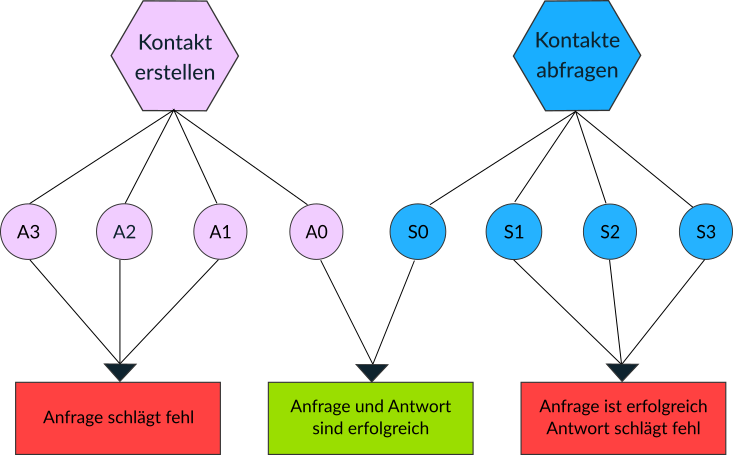
\includegraphics[width=0.8\textwidth]{Szenarien}
%   \grayRule
%   \caption[Szenarien]{Szenarien und Fälle}
%   \label{fig:scenarios}
% \end{figure}
%
% ERGEBNIS
%
\subsubsection*{Ergebnis}
Die Szenarien \it{ID0} und \it{ID1} beschreiben die Identifizierung einzelner Kontakte. Eine eindeutige Identifizierung des Kontakts ist im Szenario \it{ID0}, mittels der Verwendung einer \gls{UUID}, gewährleistet.\\
% Die Szenarien \it{V1}, \it{V2} und \it{V4}, \it{V5} beschreiben Situationen mit demselben Ausgangspunkt. In einem Fall kommt zu keinem Konflikt, in dem nächsten schon. Deswegen können \it{V1} und \it{V2}, sowie \it{V4} und \it{V5} zusammengefasst werden.
Es wird deutlich, dass es in jedem Fall zu einem Konflikt kommen kann. Es gilt zu unterscheiden in welchen Fällen mit Konflikten umgegangen werden muss weil sonst Daten verloren gehen.
\\\\
Im weiteren Verlauf dieser Arbeit werden aus dieser Erkenntnis die Anforderungen an eine offlinefähige Anwendung erarbeitet.
\chapter{\label{chap:anforderungen}Anforderungsdefinition}
Dieses Kapitel beschreibt die Anforderungen an eine Offline First Anwendung unter Berücksichtigung von Konfliktmanegement und Funktionalität.
Die von BenutzerInnen generierten Daten sollten wenigstens so lange auf dem Client gespeichert werden, bis sie vollständig beim Server angekommen sind. Jeder Fehlersfall muss kommuniziert werden. Wenn es konliktbehaftete Daten gibt muss dies mitgeteilt, und angeboten werden die Konflikte zu lösen (Welche Telefonnummer ist die richtige).\\
Aus den oben genannten \hyperref[chap:szenarien]{Szenarien} werden im Folgenden die Anforderungen hergeleitet, die eine offlinefähige Anwendung \highlight{unter Berücksichtigung von...} erfüllen soll.
\begin{enumerate}
  \item Nur die Einträge laden die ich noch nicht hab
    \subitem kostet Bandbreite und Serverarbeitszeit
    \subitem doppelt (geladen)
    \subitem dauert länger (response)
  \item Einträge identifizieren (key)
    \subitem Operationen müssen dem Objekt/Eintrag zugeordnet werden
  \item Delta berechnen
  \item lokal und auf dem Server gespeichert sein
  \item 2 Objekte mit derselben ID ? welches ist das aktuellste
  \item mehr als 2 Objekte mit derselben ID ? sortieren
  \item Liste von inhaltsbasierten Versionen muss festgelegte Länge haben
  \item Konflikte effizient speichern
  \item
\end{enumerate}
\todo{Damit ein Datensatz, wie zum Beispiel ein Adressbucheintrag, offline erreichbar sind, muss er sowohl auf dem Client, als auch auf dem Server gespeichert sein. Im aktuellen Anwendungsfall bedeutet das, es gibt zwei Kopien des Adressbucheintrags. Eine auf dem Anwendungsgerät, eine auf dem Server.\\
Um dieses Delta zu kalkulieren müssen Daten auf dem Client gespeichert werden (localStorage, lokale Datenbank oder Datei...) | Server muss die Daten sortieren können und in der Lage sein nur bestimmte Daten zu liefern.}
%
% Use Cases  \hyperref[sec:conflict]{oben}
%
\section{Anwendungsfälle}
Aus den in Kapitel \ref{chap:szenarien} erarbeiteten Szenarien ergeben sich die folgenden Use-Cases, die von einer offlinefähigen Anwendung erfüllt werden sollen. Die folgende Tabelle zeigt die Anwendungsfälle aus der Entwicklungsperspektive.
\begin{longtable}[c]{@{}
>{\columncolor[HTML]{CFFCC2}}l ll@{}}
\toprule
    \multicolumn{1}{p{0.1\textwidth}}{\cellcolor[HTML]{cffcc2}\textbf{ID}}
    & \multicolumn{1}{p{0.45\textwidth}}{\cellcolor[HTML]{cffcc2}\textbf{Anwendungsfall}}
    & \multicolumn{1}{p{0.45\textwidth}}{\cellcolor[HTML]{cffcc2}\textbf{Beschreibung}}\\ \hline
\endfirsthead
%
\endhead
%
  \multicolumn{1}{l}{\cellcolor[HTML]{cffcc2}\textbf{UC1}} &
  \multicolumn{1}{p{0.45\textwidth}}
  {Um die Anwendung auch ohne Internetzugang zu nutzen, sollen die Daten auch offline erreichbar sein.}
  & \multicolumn{1}{p{0.45\textwidth}}
  {Die Daten werden auf dem Server und lokal gespeichert. Lokal bedeutet in einer lokalen Datenbank oder im Browser (localStorage, IndexedDB usw.).}\\
  \midrule
  %
  \multicolumn{1}{l}{\cellcolor[HTML]{cffcc2}\textbf{UC2}} &
  \multicolumn{1}{p{0.45\textwidth}}
  {Die Anwendung soll die Kontaktliste schnell und effizient laden.}
  % {Um Datentraffic und Ladezeiten zu sparen / schnell und effizient möchte ich nur die Adressbucheinträge oder deren Aktualisierungen laden, die sich nicht schon auf dem Endgerät befinden.}
  & \multicolumn{1}{p{0.45\textwidth}}
  % {Es wird ermittelt welche Daten neu angelegt oder aktualisiert wurden. Dazu müssen sie sortierbar und versionierbar sein.}\\
  {Es werden nur Einträge oder deren Aktualisierungen geladen, die sich noch nicht auf dem Endgerät befinden.}\\
  \midrule
  %
  \multicolumn{1}{l}{\cellcolor[HTML]{cffcc2}\textbf{UC3}} &
  \multicolumn{1}{p{0.45\textwidth}}
  {Ich möchte Einträge immer und überall editieren können.}
  & \multicolumn{1}{p{0.45\textwidth}}
  {Jeder Eintrag muss identifizierbar und versionierbar sein.}\\
  \midrule
  %
  \multicolumn{1}{l}{\cellcolor[HTML]{cffcc2}\textbf{UC4}} &
  \multicolumn{1}{p{0.45\textwidth}}
  {Um jedem Adressbucheintrag Operationen zuzuweisen und einzelne Kontakte zu finden, möchte ich die Einträge identifizieren.}
  & \multicolumn{1}{p{0.45\textwidth}}
  {Jeder Eintrag bekommt zur eindeutigen Identifikation eine \gls{UUID} zugewiesen.}\\
  \midrule
  %
  \multicolumn{1}{l}{\cellcolor[HTML]{cffcc2}\textbf{UC5}} &
  \multicolumn{1}{p{0.45\textwidth}}
  {Um zu wissen ob, wie oft und wann ein Eintrag bearbeitet wurde, möchte ich die Einträge versionieren.}
  & \multicolumn{1}{p{0.45\textwidth}}
  {Jeder Eintrag bekommt ein Versionsattribut.}\\
  \midrule
  % UC6
  \multicolumn{1}{l}{\cellcolor[HTML]{cffcc2}\textbf{UC6}} &
  \multicolumn{1}{p{0.45\textwidth}}
  {Ich möchte dass alle Änderungen ankommen und keine Daten verloren gehen.}
  &
  \multicolumn{1}{p{0.45\textwidth}}
  {Wenn ein Konflikt auftritt, wird er effizient gespeichert (statt eine Version zu verwerfen).}\\
  \midrule
  % UC7
  \multicolumn{1}{l}{\cellcolor[HTML]{cffcc2}\textbf{UC7}} &
  \multicolumn{1}{p{0.45\textwidth}}
  {Ich weiß, Konflikte können immer auftreten, deswegen möchte ich mit ihnen umgehen können.}
  & \multicolumn{1}{p{0.45\textwidth}}
  {Konflikte werden effizient gespeichert, sodass sie nach und nach von NutzerInnen aufgelöst werden können.}\\
  % end
  \bottomrule \cellcolor[HTML]{FFFFFF}
  \vspace{0.1cm}\\
  \noalign{\hspace{0.0525\textwidth}\grayRule}
  \caption{Anwendungsfälle}
  \label{tab:uc}\\
\end{longtable}

Das in Abbildung \ref{fig:uc} gezeigte Use-Case-Diagramm veranschaulicht die in der obigen Tabelle \ref{tab:uc} aufgeführten Anwendungsfälle.
\begin{figure}[H]
    \centering
    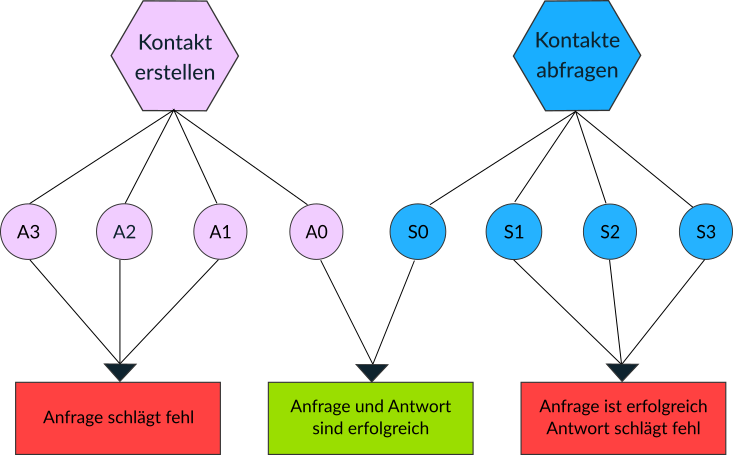
\includegraphics[width=\textwidth]{Szenarien}
    \grayRule
    \caption[Use-Case Diagramm]{Platzhalter für UC-Diagramm}
    \label{fig:uc}
\end{figure}
%
% Funktionalität
%
\section{Funktionalität}
\todo{siehe Anforderungen PWA?} Plus kein Datenverlust, und 'just work'\\
Daten sollen, sobald einmal geladen, auch offline verfügbar sein.
Daten sollen jederzeit (offline und online) lesbar und bearbeitbar (löschbar) sein.
%
% UI
%
\section{Die graphische Oberfläche}
\Gls{optimistic UI}
\gls{UI} soll mich nicht mit Meldungen darüber nerven, dass ich offline bin. (Bsp. Chat)\\
\gls{UI} soll sagen wenn es einen Konflikt gab / gibt und mich entscheiden lassen. Bzw ihn lösen lassen.
Auf keinen Fall selber lösen und mich nichts davon wissen lassen.\\
Im besten Fall soll due UI mir sagen \b{warum} es zum Konflikt gekommen ist.
%\chapter{\label{chap:implementierung}Vorgehen}
\begin{itemize}
  \item was verspricht redux-offline
  \item Wie funktioniert redux-offline? Welche Strategie zur Konfliktlösung wird verwendet?
  \item was könte daran problematisch sein?
  \item Wie hoch ist der Implementierungsaufwand?
  \item Dasselbe für Couch \& Pouch
\end{itemize}

Implementierungsaufwand: Anforderungen an Simulator? Konzeption? usw.

%\chapter{\label{chap:fazit}Zusammenfassung und Ausblick}
Interessant wäre es andere Datenbanklösungen zu untersuchen.
Realm ist leider kostenpflichtig, wäre aber äußerst spannend weil Realm so viel verspricht.

%
%	APPENDICES
%

%% Ein kleiner Abstand zu den Kapiteln im Inhaltsverzeichnis (toc)
\addtocontents{toc}{\protect\vspace*{\baselineskip}}


\printglossary[type=\acronymtype, title=Abkürzungen, style=super]
\printglossary[type=main,style=altlist]

%
%Abbildungsverzeichnis
%
\clearpage
\addcontentsline{toc}{chapter}{Abbildungsverzeichnis}
\listoffigures

% \renewcommand\lstlistlistingname{Quellcodeverzeichnis}
%\lstlistoflistings%quellcodeverzeichnis

%
% Literaturverzeichnis
%
\addcontentsline{toc}{chapter}{Literaturverzeichnis}
\bibliographystyle{alphadin}
\bibliography{extra/literatur}

%
% Anhang
%
\clearpage
\appendix
\addcontentsline{toc}{chapter}{Anhang}
\chapter*{Anhang}
\section*{Eidesstattliche Erklärung}
\section*{CD-Inhalt}
Auf der beigefügten CD befinden sich
\begin{itemize}
	\item Die schriftliche Ausarbeitung dieser Masterrarbeit im PDF-Format
	\item Das erstellte Projekt
\end{itemize}

\end{document}
